%% LyX 2.3.6.1 created this file.  For more info, see http://www.lyx.org/.
%% Do not edit unless you really know what you are doing.
\documentclass[11pt,american,czech]{book}
\usepackage[T1]{fontenc}
\usepackage[utf8]{inputenc}
\usepackage[a4paper]{geometry}
\geometry{verbose,tmargin=4cm,bmargin=3cm,lmargin=3cm,rmargin=2cm,headheight=0.8cm,headsep=1cm,footskip=0.5cm}
\pagestyle{headings}
\setcounter{secnumdepth}{3}
\usepackage{url}
\usepackage{amsmath}
\usepackage{amsthm}
\usepackage{amssymb}
\usepackage{graphicx}
\usepackage{setspace}
\usepackage{romannum}
\usepackage{caption}
\usepackage{subcaption}
\AtBeginDocument{\pagenumbering{arabic}}

\makeatletter
%%%%%%%%%%%%%%%%%%%%%%%%%%%%%% Textclass specific LaTeX commands.
\newenvironment{lyxlist}[1]
	{\begin{list}{}
		{\settowidth{\labelwidth}{#1}
		 \setlength{\leftmargin}{\labelwidth}
		 \addtolength{\leftmargin}{\labelsep}
		 \renewcommand{\makelabel}[1]{##1\hfil}}}
	{\end{list}}

%%%%%%%%%%%%%%%%%%%%%%%%%%%%%% User specified LaTeX commands.
%% Font setup: please leave the LyX font settings all set to 'default'
%% if you want to use any of these packages:

%% Use Times New Roman font for text and Belleek font for math
%% Please make sure that the 'esint' package is turned off in the
%% 'Math options' page.
\usepackage[varg]{txfonts}

%% Use Utopia text with Fourier-GUTenberg math
%\usepackage{fourier}

%% Bitstream Charter text with Math Design math
%\usepackage[charter]{mathdesign}

%%---------------------------------------------------------------------

%% Make the multiline figure/table captions indent so that the second
%% line "hangs" right below the first one.
%\usepackage[format=hang]{caption}

%% Indent even the first paragraph in each section
\usepackage{indentfirst}

%%---------------------------------------------------------------------

%% Disable page numbers in the TOC. LOF, LOT (TOC automatically
%% adds \thispagestyle{chapter} if not overriden
%\addtocontents{toc}{\protect\thispagestyle{empty}}
%\addtocontents{lof}{\protect\thispagestyle{empty}}
%\addtocontents{lot}{\protect\thispagestyle{empty}}

%% Shifts the top line of the TOC (not the title) 1cm upwards 
%% so that the whole TOC fits on 1 page. Additional page size
%% adjustment is performed at the point where the TOC
%% is inserted.
%\addtocontents{toc}{\protect\vspace{-1cm}}

%%---------------------------------------------------------------------

% completely avoid orphans (first lines of a new paragraph on the bottom of a page)
\clubpenalty=9500

% completely avoid widows (last lines of paragraph on a new page)
\widowpenalty=9500

% disable hyphenation of acronyms
\hyphenation{CDFA HARDI HiPPIES IKEM InterTrack MEGIDDO MIMD MPFA DICOM ASCLEPIOS MedInria}

%%---------------------------------------------------------------------

%% Print out all vectors in bold type instead of printing an arrow above them
\renewcommand{\vec}[1]{\boldsymbol{#1}}

% Replace standard \cite by the parenthetical variant \citep
%\renewcommand{\cite}{\citep}

\makeatother

\usepackage{babel}

\def\NameOfThesisCzech{Robustní strojové učení a adversariální vzorky}
\def\NameOfThesisEnglish{Robust machine learning and adversarial examples}
\def\NameOfAuthor{Pavel Jakš}
\def\NameOfSupervisor{Mgr. Lukáš Adam, Ph.D.}

\begin{document}
\def\documentdate{7. \v{c}ervence 2022}

%%\def\documentdate{\today}

\pagestyle{empty}
{\centering

\noindent %
\begin{minipage}[c]{3cm}%
\noindent \begin{center}

\includegraphics[width=3cm,height=3cm,keepaspectratio]{Images/TITLE/cvut}
\par\end{center}%
\end{minipage}%
\begin{minipage}[c]{0.6\linewidth}%
\begin{center}
\textsc{\large{}České vysoké učení technické v Praze}{\large{}}\\
{\large{}Fakulta jaderná a fyzikálně inženýrská}
\par\end{center}%
\end{minipage}%
\begin{minipage}[c]{3cm}%
\noindent \begin{center}

\includegraphics[width=3cm,height=3cm,keepaspectratio]{Images/TITLE/fjfi}
\par\end{center}%
\end{minipage}

\vspace{3cm}

\textbf{\huge{}\NameOfThesisCzech}{\huge\par}

\vspace{1cm}

\selectlanguage{american}%
\textbf{\huge{}\NameOfThesisEnglish}{\huge\par}

\selectlanguage{czech}%
\vspace{2cm}

{\large{}Bakalářská práce}{\large\par}

}

\vfill{}

\begin{lyxlist}{MMMMMMMMM}
\begin{singlespace}
\item [{Autor:}] \textbf{\NameOfAuthor}
\item [{Vedoucí~práce:}] \textbf{\NameOfSupervisor}
%\item [{Konzultant:}] \textbf{doc. RNDr. Jméno Konzultanta, CSc. }(pouze pokud konzultant byl jmenován.)
\item [{Akademický~rok:}] 2021/2022
\end{singlespace}
\end{lyxlist}
\newpage{}

~\newpage{}

~

\vfill{}

\begin{center}
- Zadání práce -
\par\end{center}

\vfill{}

~\newpage{}

~

\vfill{}

\begin{center}
- Zadání práce (zadní strana) -
\par\end{center}

\vfill{}

~\newpage{}

\noindent \emph{\Large{}Poděkování:}{\Large\par}

\noindent Chtěl bych zde poděkovat především svému školiteli - panu doktoru Adamovi -
za pečlivost, ochotu, vstřícnost a odborné i lidské zázemí při vedení
mé bakalářské práce.

\vfill

\noindent \emph{\Large{}Čestné prohlášení:}{\Large\par}

\noindent Prohlašuji, že jsem tuto práci vypracoval samostatně a uvedl
jsem všechnu použitou literaturu.

\bigskip{}

\noindent V Praze dne \documentdate\hfill{}\NameOfAuthor

\vspace{2cm}

\newpage{}

~\newpage{}

\begin{onehalfspace}
\noindent \emph{Název práce:}

\noindent \textbf{\NameOfThesisCzech}
\end{onehalfspace}

\bigskip{}

\noindent \emph{Autor:} \NameOfAuthor

\bigskip{}

\noindent \emph{Obor:} Matematická informatika\bigskip{}

% \noindent \emph{Zaměření:} Celý název zaměření (Pokud obor neobsahuje zaměření, tuto řádku odstranit.)

\bigskip{}

\noindent \emph{Druh práce:} Bakalářská práce

\bigskip{}

\noindent \emph{Vedoucí práce:} \NameOfSupervisor,
Katedra počítačů,
Fakulta elektrotechnická,
České vysoké učení technické v Praze,
Karlovo náměstí 13, 121 35, Praha 2

\bigskip{}

% \noindent \emph{Konzultant:} doc. RNDr. Jméno Konzultanta, CSc., pracoviště
% konzultanta. Pouze pokud konzultant byl jmenován.

\bigskip{}

\noindent \emph{Abstrakt:} Abstrakt max. na 10 řádků. Abstrakt max.
na 10 řádků. Abstrakt max. na 10 řádků. Abstrakt max. na 10 řádků.
Abstrakt max. na 10 řádků. Abstrakt max. na 10 řádků. Abstrakt max.
na 10 řádků. Abstrakt max. na 10 řádků. Abstrakt max. na 10 řádků.
Abstrakt max. na 10 řádků. Abstrakt max. na 10 řádků. Abstrakt max.
na 10 řádků. Abstrakt max. na 10 řádků. Abstrakt max. na 10 řádků.
Abstrakt max. na 10 řádků. Abstrakt max. na 10 řádků. Abstrakt max.
na 10 řádků. Abstrakt max. na 10 řádků. Abstrakt max. na 10 řádků.
Abstrakt max. na 10 řádků. Abstrakt max. na 10 řádků. Abstrakt max.
na 10 řádků. Abstrakt max. na 10 řádků. Abstrakt max. na 10 řádků.
Abstrakt max. na 10 řádků. Abstrakt max. na 10 řádků. Abstrakt max.
na 10 řádků. Abstrakt max. na 10 řádků. Abstrakt max. na 10 řádků. 

\bigskip{}

\noindent \emph{Klíčová slova:} klíčová slova (nebo výrazy) seřazená
podle abecedy a oddělená čárkou

\vfill{}
~

\selectlanguage{american}%
\begin{onehalfspace}
\noindent \emph{Title:}

\noindent \textbf{\NameOfThesisEnglish}
\end{onehalfspace}

\bigskip{}

\noindent \emph{Author:} \NameOfAuthor

\bigskip{}

\noindent \emph{Abstract:} Max. 10 lines of English abstract text.
Max. 10 lines of English abstract text. Max. 10 lines of English abstract
text. Max. 10 lines of English abstract text. Max. 10 lines of English
abstract text. Max. 10 lines of English abstract text. Max. 10 lines
of English abstract text. Max. 10 lines of English abstract text.
Max. 10 lines of English abstract text. Max. 10 lines of English abstract
text. Max. 10 lines of English abstract text. Max. 10 lines of English
abstract text. Max. 10 lines of English abstract text. Max. 10 lines
of English abstract text. Max. 10 lines of English abstract text.
Max. 10 lines of English abstract text. Max. 10 lines of English abstract
text. Max. 10 lines of English abstract text. Max. 10 lines of English
abstract text. Max. 10 lines of English abstract text. Max. 10 lines
of English abstract text. Max. 10 lines of English abstract text.
Max. 10 lines of English abstract text. Max. 10 lines of English abstract
text. Max. 10 lines of English abstract text.

\bigskip{}

\noindent \emph{Key words:} keywords in alphabetical order separated
by commas

\selectlanguage{czech}%
\newpage{}

~\newpage{}

\pagestyle{plain}

\tableofcontents{}

\newpage{}

\chapter*{Úvod}

\addcontentsline{toc}{chapter}{Úvod}

Pojem neuronové sítě představuje výpočetní jednotku, která svou univerzálností nachází uplatnění v~mnoha disciplínách.

% \pagestyle{headings}

% Neuronové sítě
\chapter{Neuronové sítě}

Neuronová síť je svým charakterem velmi přizpůsobivý výpočetní stroj vhodný pro řešení mnoha problémů.
Mezi nejčastější problémy, jejichž řešením může být vhodná neuronová síť, patří \emph{regrese},
čili předpovídání jedné skalární hodnoty na základě vstupu,
či \emph{klasifikace}, která má za cíl předpovědět třídu v němž se daný vstup nachází.
Obecně tak neuronové síti odpovídá libovolně komplikované zobrazení
$F: \mathbb{R}^{n_1 \times ... \times n_k} \rightarrow \mathbb{R}^{m_1 \times ... \times m_l}$.
Pro případ regrese potom $l = 1$, $m_1 = 1$ a výstup $F$ hraje roli predikované hodnoty,
pro případ klasifikace je též $l = 1$,
ale $m_1$ je rovno počtu tříd a výstup $F$ je predikovanou pravděpodobnostní distribucí,
která určuje s jakou pravděpodobností patří daný vstup příslušné třídě.

Samotná síť sestává z mnoha dílčích navzájem propojených částí,
o nichž pojednávají následující pasáže této kapitoly.

\section{Vrstva neuronů}

Prvním základním konceptem, který stojí za pojmem neuronové sítě, je rozdělení výpočtu do vrstev.
Takové vrstvy potom charakterizuje zobrazení
$\phi : \mathbb{R}^{p_1 \times ... \times p_r} \rightarrow \mathbb{R}^{q_1 \times ... \times q_s}$,
jehož předpis již lze snadno vyjádřit.
Obrazy vstupů při zobrazení $\phi$ se potom nazývají \emph{aktivace}.

\subsection{Hustá vrstva}

Prvním příkladem vrstev neuronů je tzv. \emph{hustá vrstva}
(angl. \emph{dense layer} nebo \emph{fully-connected layer}).
Pro zobrazení $\phi$ platí, že zobrazuje vektory na vektory, tedy $r = s = 1$,
a má předpis
\begin{equation} \label{dense}
	\phi (u) = W u + b,
\end{equation}
kde $W \in \mathbb{R}^{q_1 \times p_1}$ je \emph{matice vah} (z angl. \emph{weight})
a $b \in \mathbb{R}^{q_1}$ je \emph{vektor prahů} (z angl. \emph{bias}).

Motivací za pojmenováním této vrstvy jako husté nebo též plně propojené je fakt,
že každá složka vstupujícího vektoru ovlivňuje každou z výsledných aktivací,
pokud tedy příslušný prvek matice vah není nulový.

\subsection{Konvoluční vrstva}

Pro představení dalšího typu vrstvy uvěďme základní přehled o operaci konvoluce.
Operace \emph{konvoluce} je ve vší obecnosti operace mezi dvěma číselnými funkcemi $g$ a $h$ se stejným definičním oborem,
jejíž výstupem je nová číselná funkce standardně označovaná jako $g*h$.
Uveďme zde definici konvoluce pro reálné funkce definované na $\mathbb{R}^d$,
tedy $g,h: \mathbb{R}^d \rightarrow \mathbb{R}$:
\begin{equation*}
	(g * h)(t) = \int_{\mathbb{R}^{d}} g(\tau) h(t - \tau) d\tau.
\end{equation*}
Důležitým předpokladem pro možnost konvoluce je samozřejmě existence integrálu na pravé straně.

Ačkoliv je konvoluce komutativní operací,
nejen v kontextu strojového učení se mezi oběma funkcemi vstupujícími do konvoluce rozlišuje.
Funkce vstupující jako první se nazývá vstup a druhá funkce se nazývá jádrem.
Dále se v kontextu konvolučních sítí standardně objevují diskrétní funkce,
které nabývají nenulových hodnot pouze v konečně mnoha bodech.
Potom integrál přes $\mathbb{R}^d$ přechází v konečnou sumu:
\begin{equation}
	(g * h)(i_1, ..., i_d) = \sum_{j_1} ... \sum_{j_d} g(j_1, ..., j_d) h(i_1 - j_1, ..., i_d - j_d).
\end{equation}
Díky komutativitě konvoluce lze též psát:
\begin{equation}
	(g * h)(i_1, ..., i_d) = \sum_{j_1} ... \sum_{j_d} g(i_1 - j_1, ..., i_d - j_d) h(j_1, ..., j_d).
\end{equation}
Při aplikaci komutativity došlo k tzv. \emph{překlopení jádra} (termín pochází z anglického kernel flipping).
Za~vynechání překlopení jádra lze dojít ke \emph{křížové korelaci}:
\begin{equation}
	(g * h)(i_1, ..., i_d) = \sum_{j_1} ... \sum_{j_d} g(i_1 + j_1, ..., i_d + j_d) h(j_1, ..., j_d).
\end{equation}
Mnoho knihoven zabývajících se neuronovými sítěmi dle \cite{Goodfellow} implementují křížovou korelaci namísto konvoluce,
ačkoliv tuto svou implementaci nazývají konvolucí.

Nejčastější užití konvoluce v neuronových sítích je při zpracování obrázků,
které lze reprezentovat pomocí $C \times W \times H$ tenzorů,
kde $C$ značí počet kanálů obrázku (nejčastěji tři pro červenou, zelenou a modrou),
$W$ je šířka, $H$ je výška obrázku.
Uvěďme předpis pro zobrazení $\phi$, které odpovídá konvoluční vrstvě:
\begin{equation} \label{convolution_layer}
	\forall j \in \{1, 2, ..., C_{out}\} \qquad \phi(u)_j = b_j + \sum_{i=1}^{C_{in}} K_{j, i} * u_i
\end{equation}
kde $\phi : \mathbb{R}^{C_{in} \times W_{in} \times H_{in}} \rightarrow \mathbb{R}^{C_{out} \times W_{out} \times H_{out}}$
($C_{in}$ je počet vstupních kanálů, $C_{out}$ počet výstupních kanálů,
$W_{in}$, $H_{in}$ jsou vstupní šířka a výška, $W_{out}$, $H_{out}$ jsou výstupní šířka a výška),
$b \in \mathbb{R}^{C_{out} \times W_{out} \times H_{out}}$ je práh,
$K~\in~\mathbb{R}^{C_{out} \times C_{in} \times k_1 \times k_2}$
je tenzor konvolučních jader ($k_1$ a $k_2$ jsou rozměry konvolučního jádra).

Za povšimnutí stojí, že standardně $W_{out} \neq W_{in}$ a $H_{out} \neq H_{in}$,
konkrétně při takto prosté implementaci konvoluční vrstvy platí:
\begin{align}
	W_{out} &= W_{in} - k_1 + 1, \\
	H_{out} &= H_{in} - k_2 + 1.
\end{align}

\subsection{Pooling vrstva}

Pojem \emph{pooling vrstvy} (bez překladu) se skrývá funkce,
která reportuje souhrné statistiky vstupu.
Například nejčastěji používanou pooling vrstvou je tzv. \emph{max pooling}
s parametry $k_1$, $k_2$ (angl. \emph{kernel-size}),
která při aplikaci na obrázek o rozměrech $C \times W_{in} \times H_{in}$ (počet kanálů, šířka, výška)
v každém kanálu reportuje maximální hodnotu v blocích o rozměrech $k_1 \times k_2$.
Potom zobrazení $\phi$ je zobrazení $\phi:\mathbb{R}^{C \times W_{in} \times H_{in}}~\rightarrow~\mathbb{R}^{C \times W_{out} \times H_{out}}$,
kde platí:
\begin{align}
	W_{out} &= \left\lceil \frac{W_{in}}{k_1} \right\rceil, \\
	H_{out} &= \left\lceil \frac{H_{in}}{k_2} \right\rceil,
\end{align}
a má předpis $\forall i \in \{1, ..., C\}, \forall j \in \{1, ..., W_{out}\}, \forall k \in \{1, ..., H_{out}\}$:
\begin{equation}
	\phi(u)_{i, j, k} = \operatorname{max}\{u_{i, \mu, \nu} | (j-1) k_1 < \mu \leq j k_1, (k-1) k_2 < \nu \leq k k_2 \}.
\end{equation}

\subsection{Aktivační vrstva}

\emph{Aktivační vrstva} označuje vrstvu, která slouží k omezení aktivací jiné vrstvy,
aby byly v rozumných mezích. Např. jedná-li se o poslední vrstvu klasifikační neuronové sítě,
pak aktivační vrstva zajišťuje, aby výsledné aktivace byly pravděpodobnostní distribucí.

Mezi často používané aktivační vrstvy patří funkce, jež vzniknou aplikací skalární funkce 
jedné proměnné $\sigma : \mathbb{R} \rightarrow \mathbb{R}$ na každý prvek vstupu zvlášť.
Pro takové skalární funkce pak máme pojem aktivační funkce.
Nejčastější aktivační funkce jsou následující:
\begin{itemize}
	\item Sigmoid: $\sigma(z) = \frac{1}{1 + e^{-z}}$,
	\item ReLU: $\sigma(z) = \operatorname{max}(0, z)$,
	\item LeakyReLU: $\sigma(z) = \operatorname{max}(0, z) + \alpha * \operatorname{min}(z, 0)$, kde $\alpha > 0$,
	\item Tanh: $\sigma(z) = tanh(z) = \frac{e^{z} - e^{-z}}{e^{z} + e^{-z}}$.
\end{itemize}

Další oblíbenou aktivační vrstvou je \emph{softmax vrstva}.
Ta má pro odpovídající funkci $\phi$, která v tomto případě zobrazuje vektor na vektor stejných rozměrů
(tedy $\phi : \mathbb{R}^{p_1} \rightarrow \mathbb{R}^{p_1}$) předpis:
\begin{equation} \label{softmax}
	\forall i \in \{1, 2, ..., p_1\} \quad \phi (u)_i = \frac{e^{u_i}}{\sum_{j=1}^{p_1} e^{u_j}}.
\end{equation}
Užití této aktivační vrstvy je nasnadě. Jelikož prvky výsledné aktivace leží v intervalu $[0, 1]$
a sečtou se na $1$, lze výstup takovéto aktivační vrstvy interpretovat jako pravděpodobnostní distribuci.

\section{Hluboká dopředná neuronová síť}

Nejjednodušším modelem neuronové sítě je \emph{hluboká dopředná neuronová síť},
která je složením hustých a aktivačních vrstev.
Konkrétně je odpovídající zobrazení $F$ složením sudého počtu vrstev,
kde na liché pozici je vrstva hustá a na sudé pozici je vrstva aktivační.
Tedy $F : \mathbb{R}^{n_1} \rightarrow \mathbb{R}^{m_1}$.

Motivace za pojmenováním takovéhoto zobrazení jako hluboké dopředné neuronové sítě je následující:
Pojmem \emph{neuronová síť} se rozumí složení každé jednotlivé dvojvrstvy
$\varphi = \phi_{activation} \circ \phi_{dense}$
(hustá vrstva $\phi_{dense}$ spojená s následující aktivační vrstvou $\phi_{activation}$)
z mnoha tzv. \emph{umělých neuronů}
- dílčích výpočetních jednotek, které mají přepis 
\begin{equation} \label{neuron}
	\varphi (u)_i = \sigma \left(b_i + \sum_{j=1}^n w_{i,j} u_j\right),
\end{equation}
kde $b_i$ je $i$-tá složka vektoru prahů husté vrstvy,
$w_{i,j}$ je složka v $i$-tém řádku a $j$-tém sloupci matice vah husté vrstvy
a $\sigma$ je aktivační funkce příslušející aktivační vrstvě.
Takto definovaný umělý neuron vzdáleně připomíná neuron v biologickém smyslu,
neboť má mnoho vstupů a jeden výstup.
Tímto způsobem zavedené umělé neurony jsou potom pospojovány v neuronovou síť.

Za pojmem \emph{dopředná} v názvu hluboká dopředná neuronová síť stojí fakt,
že informace plyne od vstupu první vrstvy až po aktivace poslední vrstvy v jediném směru,
který je určen architekturou sítě.

Termín \emph{hluboká} je potom zaveden pro sítě, které mají více než jednu dvojvrstvu.

\section{Konvoluční neuronová síť}

Pojmem \emph{konvoluční neuronová síť} je myšleno složení vrstev neuronů,
z nichž alespoň jedna je konvoluční.
Standardně je konvoluční vrstva používána společně s aktivační vrstvou a pooling vrstvou,
a tedy tvoří konvoluční trojvrstvu $\varphi = \phi_{pooling} \circ \phi_{activation} \circ \phi_{convolution}$,
kde $\phi_{convolution}$ je konvoluční vrstva,
$\phi_{activation}$ je aktivační vrstva a $\phi_{pooling}$ je pooling vrstva.
Takovýchto trojvrstev může být v konvoluční síti několik za sebou
a následovat může několik vrstev hustých spolu s aktivačními.
Takto zavedená konvoluční trojvrstva má velmi vítanou vlastnost,
totiž že výsledná síť je do určité míry invariantní vůči translacím vstupu \cite{Goodfellow}.

% Úvodní pojednání o neuronových sítích
% Umělý neuron
% Princip fungování neuronové sítě spočívá v poskládání celku z dílčích výpočetních jednotek - umělých neuronů.
% Takovýto neuron je standardně funkcí více proměnných, jehož výstup je proměnná jediná.
% Typickým modelem umělého neuronu je funkce $f: \mathbb{R}^n \rightarrow \mathbb{R}$ definovaná předpisem
% \begin{equation} \label{neuron}
% 	f(a_1, ..., a_n) = \sigma (\sum_{i=1}^n w_i a_i + b) ,
% \end{equation}
% kde \emph{n} je počet vstupujících proměnných, \emph{$w_i$} jsou tzv. váhy (w z anglického slova weight),
% \emph{b} je práh (b~z~anglického slova bias), \emph{$\sigma$} označuje tzv. aktivační funkci.

% Roli vstupujících proměnných mohou hrát např. hodnoty RGB pixelů barevných obrázků, je-li aplikací klasifikace obrázků,
% nebo výstupy jiných neuronů.
% Pod pojmem váha se skrývá míra ovlivnění výstupu neuronu daným vstupem.
% Je-li váha u nějakého vstupu vysoká, pak je výstup citlivější na daný vstup.
% Práh pro změnu určuje posunutí citlivosti neuronu na všechny vstupy jako celku.

% Poslední, avšak velmi důležitou charakteristikou tohoto modelu neuronu je aktivační funkce.
% Za aktivační funkci lze vzít libovolnou funkci $\sigma : \mathbb{R} \rightarrow \mathbb{R}$,
% existuje však základní sada:
% \begin{itemize}
% 	\item Sigmoid: $\sigma(z) = \frac{1}{1 + e^{-z}}$,
% 	\item ReLU: $\sigma(z) = max(0, z)$,
% 	\item LeakyReLU: $\sigma(z) = max(0, z) + \alpha * min(z, 0)$, kde $\alpha \in \mathbb{R}^+$,
% 	\item Tanh: $\sigma(z) = tanh(z) = \frac{e^{z} - e^{-z}}{e^{z} + e^{-z}}$.
% \end{itemize}
% Tyto funkce lze doplnit o jejich mírné modifikace.
% Moderní doporučenou praxí je užívat ReLU jako aktivační funkci a (\ref{neuron}) jako model neuronu dle \cite{Goodfellow}.


% \section{Hluboká dopředná neuronová síť}
% Je-li pojem umělého neuronu objasněn, lze se přesunout k jeho užití v neuronových sítích.
% Základní myšlenkou těchto sítí je vhodné poskládání umělých neuronů do vrstev, které dohromady tvoří síť neuronů.
% Taková vrstva je potom trojího druhu - vstupní, výstupní a skrytá.
% \emph{Vstupní vrstva} je množina umělých neuronů, které mají za vstup výstupy problému, jehož je neuronová síť řešením.
% Za vstup si lze představit matici černobílých pixelů, které představují obrázek číslice, kterou je cíl klasifikovat.
% \emph{Výstupní} vrstva sestává z neuronů, které mají za vstup výstupy neuronů předchozí vrstvy.
% Výstupem této vrstvy pak bude řešení daného problému - například klasifikace číslice.
% Posledním druhem vrstvy je \emph{vrstva skrytá}.
% Takováto vrstva má za vstupy výstupy vrstvy předcházející a její výstupy slouží jako vstupy pro~vrstvu nadcházející.
% Má-li neuronová síť tuto architekturu, hovoří se o \emph{dopředné neuronové síti}.
% Má-li navíc alespoň jednu skrytou vrstvu, lze mluvit o \emph{hluboké dopředné neuronové síti}.

% Se znalostí pojmu vrstvy neuronů lze přistoupit k poznámce o tzv. \emph{softmax funkci}.
% Jedná se o vektorovou funkci $s: \mathbb{R}^m \rightarrow \mathbb{R}^m$, kde
% \begin{equation*}
% 	s(a_1, ..., a_m)_i = \frac{e^{a_i}}{\sum_{j=1}^m e^{a_j}},
% \end{equation*}
% kde $i \in \hat{m}$.
% Její užití je nasnadě: Výstup této funkce lze totiž interpretovat jako diskrétní pravděpodobnostní distribuci,
% a proto ji lze užít jako aktivační funkci výstupní vrstvy, je-li cílem dané neuronové sítě klasifikace vstupu do kategorií.

% Další poznámka se bude věnovat zjednodušení zápisu akce vrstvy na vstup.
% Podle modelu neuronu v~(\ref{neuron}) se akce jednodnoho neuronu na vstup sestává z násobení,
% následného sčítání, přičtení prahu a aplikací aktivační funkce.
% Tato procedura nastává pro každý neuron ve vrstvě.
% Tak lze sestavit z jednotlivých vah $w_i^{(j)}$ (\emph{i}-tá váha \emph{j}-tého neuronu ve vrstvě) matici $\mathbb{A}$,
% jejímiž prvky jsou právě ony váhy $(\mathbb{A})_{j,i} = w_i^{(j)}$,
% z~prahů pak vektor $b$, jehož $j$-tá složka je rovna prahu $j$-tého neuronu.
% Dále zaveďme vektorovou funkci $s: \mathbb{R}^m \rightarrow \mathbb{R}^m$ - ať už jako výše zmíněnou softmax funkci,
% nebo jako po složkách aplikovanou libovolnou aktivační funkci $\sigma$
% ve smyslu $s(a_1, ... a_m)_i = \sigma(a_i)$ pro $i \in \hat{m}$. 
% Pak lze psát, že aplikace vrstvy neuronů je zobrazení $\phi : \mathbb{R}^n \rightarrow \mathbb{R}^m$
% působící na vektor $a$ následovně:
% \begin{equation} \label{layer}
% 	\phi(a) = s(\mathbb{A}a + b).
% \end{equation}
% Tedy stěžejní operací se stává maticové násobení, respektive násobení vektoru maticí zleva.

% Při tomto si lze povšimnout, že takováto neuronová síť má řadu parametrů, o kterých není jasné jak je správně nastavit.
% Některé parametry (například váhy a prahy) se nastavují během učení neuronové sítě, čemuž je věnována samostatná kapitola.
% Potom tu jsou parametry, jejichž charakter je poněkud odlišný.
% Jedná se o ty parametry, které zůstávají během života neuronové sítě netknuté.
% Jako příklad lze uvést počet neuronů ve skryté vrstvě, který se promítne v rozměrech matice vah či dimenzionalitě výstupu vrstvy.
% Takovýmto prametrům je přisuzován název hyper-parametry.

% \section{Konvoluční sítě}

% % Úvod do CNNs
% \emph{Konvoluční sítě} nebo též \emph{konvoluční neuronové sítě} přinášejí svou architekturou
% nové možnosti zpracování dat se specifickou strukturou, do které patří například časové řady,
% obrázky nebo videa.
% Středobodem konvolučních sítí je, jak již název napovídá, operace \emph{konvoluce}.
% Ta nahrazuje maticové násobení, kterým lze reprezentovat operace ve výše popsaném modelu hluboké dopředné sítě.

% % \subsection{Konvoluce}

% Operace \emph{konvoluce} je ve vší obecnosti operace mezi dvěma číselnými funkcemi $g$ a $h$ se stejným definičním oborem,
% jejíž výstupem je nová číselná funkce standardně označovaná jako $g*h$.
% Uveďme zde definici konvoluce pro reálné funkce definované na $\mathbb{R}^d$,
% tedy $g,h: \mathbb{R}^d \rightarrow \mathbb{R}$:
% \begin{equation*}
% 	(g * h)(t) = \int_{\mathbb{R}^{d}} g(\tau) h(t - \tau) d\tau.
% \end{equation*}
% Důležitým předpokladem pro možnost konvoluce je samozřejmě konvergence integrálu na pravé straně.

% Ačkoliv je konvoluce komutativní operací, v kontextu strojového učení se mezi oběma funkcemi vstupujícími do konvoluce rozlišuje.
% Funkce vstupující jako první se nazývá vstup a druhá funkce se nazývá jádrem.
% Dále se v kontextu konvolučních sítí standardně objevují diskrétní funkce,
% které nabývají nenulových hodnot pouze v konečně mnoha bodech.
% Potom integrál přes $\mathbb{R}^d$ přechází v konečnou sumu:
% \begin{equation}
% 	(g * h)(i_1, ..., i_d) = \sum_{j_1} ... \sum_{j_d} g(j_1, ..., j_d) h(i_1 - j_1, ..., i_d - j_d).
% \end{equation}
% Díky komutativitě konvoluce lze též psát:
% \begin{equation}
% 	(g * h)(i_1, ..., i_d) = \sum_{j_1} ... \sum_{j_d} g(i_1 - j_1, ..., i_d - j_d) h(j_1, ..., j_d).
% \end{equation}
% Při aplikaci komutativity došlo k tzv. \emph{překlopení jádra} (termín pochází z anglického kernel flipping).
% Za~vynechání překlopení jádra lze dojít ke \emph{křížové korelaci}:
% \begin{equation}
% 	(g * h)(i_1, ..., i_d) = \sum_{j_1} ... \sum_{j_d} g(i_1 + j_1, ..., i_d + j_d) h(j_1, ..., j_d).
% \end{equation}
% Mnoho knihoven zabývajících se neuronovými sítěmi dle \cite{Goodfellow} implementují křížovou korelaci namísto konvoluce,
% ačkoliv tuto svou implementaci nazývají konvolucí.

% % \subsection{Pooling}
% Další nedílnou součástí konvolučních sítí je tzv. \emph{pooling}.
% Spolu s konvolucí tvoří mocný nástroj, který ve formě konvolučních a pooling vrstev hlubokých neuronových sítí
% přináší například invarianci sítě vůči malému posunutí vstupu (dle \cite{Goodfellow}).

% Pooling je funkce, která nahrazuje hodnoty v bodech nějakou souhrnou statistikou určitého okolí daného bodu.
% Např. \emph{max pooling} aplikovaný na matici se podívá na obdélníkové okolí předem definovaných rozměrů daného bodu
% a jako svůj výstup vybere maximální hodnotu nalezenou v onom okolí.
% Jiné oblíbené pooling funkce zahrnují funkce reportující průměr či $L^2$ normu daného obdelníkového okolí.

% Standardní konvoluční vrstva neuronové sítě pak sestává ze tří fází.
% První fáze provádí paralelně několik konvolucí, které produkují sadu aktivcí.
% Druhá fáze, někdy označovaná jako \emph{detekční fáze}, aplikuje na výstupy první fáze aktivační funkci.
% Třetí fáze potom provádí \emph{pooling}.

% Učení neuronové sítě
\chapter{Učení neuronové sítě}

Předchozí kapitola představila neuronové sítě jakožto složení vrstev neuronů.
Jednotlivé vrstvy jsou ovšem parametrizovány parametry, o nichž není jasné, jak je nastavit.
Například hustá vrstva má za parametry matici vah $W$ a vektor prahů $b$.
Označme tedy písmenem $\theta$ vektor všech parametrů neuronové sítě
a poznamenejme závislost zobrazení neuronové sítě na parametrech $\theta$ dolním indexem v $F_\theta$.
Hledání vhodných parametrů $\theta$ je potom označováno pojmem \emph{učení neuronové sítě}.

Standardní přístup k učení je paradigma učení s učitelem.
Tento pohled na učení neuronové sítě předpokládá existenci
tzv. \emph{trénovací sady dat} $\mathbb{T}$ (angl. \emph{training dataset}),
což je uspořádaná dvojice obsahující množinu \emph{vzorků} $\mathbb{X} = \left\{x^{(i)} | i \in \{1, ..., N\} \right\}$
a k nim příslušné \emph{značky} $\mathbb{Y} = \left\{y^{(i)} | i \in \{1, ..., N\} \right\}$,
kde pojem vzorek představuje vstup neuronové sítě
a pojem značka představuje správný výstup neuronové sítě;
$N$ je potom velikost trénovací sady $\mathbb{T}$.
Trénovací sada pak hraje roli učitele.

\section{Účelové funkce}

Je-li pojem trenovací sady objasněn, lze přistoupit k termínu \emph{účelové funkce}
nebo též \emph{ztrátové funkce}.
Jedná se o reálnou funkci, která měří, jak moc se trénovaná neuronová síť mýlí
ve svých predikcích na~vzorcích trénovací sady.
Úloha učení je potom převedena na úlohu optimalizace tohoto vhodně zvoleného kritéria.

Standardní účelová funkce je sestavena jako průměr dílčích ztrát,
které neuronová síť dosahuje na vzorcích trénovací sady:
\begin{equation} \label{averageloss}
	J(\theta) = \frac{1}{N} \sum_{i=1}^N L\left(F_{\theta}(x^{(i)}), y^{(i)}\right),
\end{equation}
kde $L$ značí konkrétní ztrátu pro daný vzorek a $J$ je celková účelová funkce.

\subsection{Střední kvadratická chyba}

Jedna z klasických účelových funkcí je funkce \emph{střední kvadratické chyby}.
Je dána přepisem:
\begin{equation} \label{mean_square_error}
	J(\theta) = \frac{1}{N} \sum_{i=1}^N \|F_\theta(x^{(i)}) - y^{(i)}\|_2^2,
\end{equation}
kde $\|\cdot\|_2$ je $l_2$ norma.

Výhodou této účelové funkce je fakt, že ji lze aplikovat na tenzory libovoných rozměrů.
Nahlédneme-li na výraz v \eqref{mean_square_error}, $J(\theta)$ nabývá vždy nezáporné hodnoty
a globální minimum $0$ právě tehdy, když pro každý vzorek trénovací datové sady je předpověď neuronové sítě správná.

Další vlastností této účelové funkce je rozdíl v citlivosti na malé hodnoty výrazu $|F_\theta(x^{(i)})_j - y^{(i)}_j|^2$,
ze kterých výsledná $l_2$ norma sestává,
oproti jeho velkým hodnotám. Tj. pro $|F_\theta(x^{(i)})_j - y^{(i)}_j| < 1$ je výraz po umocnění na druhou ještě menší,
kdežto pro $|F_\theta(x^{(i)})_j - y^{(i)}_j| > 1$ je výraz po umocnění ještě větší,
což při aplikaci později popsaných algoritmů minimalizace ztráty, které využívají gradient účelové funkce,
vede k větší toleranci malých odchylek, než kdyby byla použita $l_1$ norma.


\subsection{Ztráta křížové entropie}

Pro klasifikační problémy se ovšem standardně používá \emph{ztráta křížové entropie}.
Připomeňme, že u klasifikačního problému je výstup neuronové sítě pravděpodobnostní distribuce
a značky jsou též pravděpodobnostní distribuce.
Křížová entropie potom měří vzdálenost distribučních funkcí
a má svůj původ v \emph{Kullbackově-Leiblerově divergenci} $D_{KL}$.
Máme-li dvě pravděpodobnostní distribuce $f$ a $g$,
pak křížová entropie $H(f, g)$ je rovna
\begin{equation}
	H(f, g) = H(f) + D_{KL}(f, g),
\end{equation}
kde $H(f)$ je entropie $f$.
Pro diskrétní pravděpodobnostní distribuce máme:
\begin{equation}
	H(f, g) = - \sum_i f_i \operatorname{ln}(f_i) + \sum_i f_i \operatorname{ln} \left(\frac{f_i}{g_i}\right)
	= - \sum_i f_i \operatorname{ln}(g_i).
\end{equation}


Proto lze psát:
\begin{equation} \label{crossentropy}
	J(\theta) = \frac{1}{N} \sum_{i=1}^N H(y^{(i)}, F_\theta(x^{(i)})).
\end{equation}
Onen výraz $H(y^{(i)}, F_\theta(x^{(i)}))$ v (\ref{crossentropy}) lze tedy spočíst následovně:
\begin{equation}
	H(y^{(i)}, F_\theta(x^{(i)})) = - \sum_{j=1}^m y^{(i)}_j \cdot \ln (F_\theta(x^{(i)})_j).
\end{equation}

% Zmiňme důležitost přechodu od Kullbackovy-Leiblerovy divergence ke křížové entropii.
% Standardně je značka $y$ v tzv. \emph{one-hot encoding} formě,
% tedy je nulová až na jednu komponentu, která je rovna $1$.
% Potom by dle definice $D_{KL}(y, F_\theta(x))$ byla ona divergence nedefinovaná,
% neboť bychom měli sčítat výrazy $0 \cdot \operatorname{ln}(0)$.


% Aby bylo možné zadefinovat učeovou funkci pomocí \emph{záporného logaritmu věrohodnosti} (ZLV),
% je nutné uvést na scénu jiný pohled na neuronové sítě, a to jako na statistický model.
% Tento model potom určuje pravděpodobnost pozorování daných hodnot $y^{(i)}$ za podmínky, že vstupem je $x^{(i)}$ a parametry modelu jsou $\theta$.
% Cílem učení je potom nalezení vhodných parametrů $\theta$.
% Myšlenka je, že nejvhodnějšími parametry $\theta$ budou ty parametry, které maximalizují pravděpodobnost, že při $x^{(1)}$, ... $x^{(N)}$
% jakožto vzorcích dojde k napozorování značek $y^{(1)}$, ... $y^{(N)}$.
% Provádí se tedy bodový odhad parametrů modelu odhadem maximální věrohodnosti.
% Cílené parametry lze potom za předpokladu nezávislosti výběru vzorků získat jako:
% \begin{equation}
% 	\hat{\theta} = \arg\max_{\theta} \prod_{i=1}^N P[y^{(i)}|x^{(i)}; \theta]
% \end{equation}
% S takovýmto součinem je ovšem pracné nakládat, proto lze využít vlastností přirozeného logaritmu a problém přeformulovat následovně:
% \begin{equation}
% 	\hat{\theta} = \arg\max_{\theta} \sum_{i=1}^N \ln P[y^{(i)}|x^{(i)}; \theta]
% \end{equation}
% Aby byl problém formulován jako minimalizační, je nutné před sumu vložit jedno mínus:
% \begin{equation}
% 	\hat{\theta} = \arg\min_{\theta} - \sum_{i=1}^N \ln P[y^{(i)}|x^{(i)}; \theta]
% \end{equation}

% Pro úkol klasifikce, kdy výstupem neuronové sítě je diskrétní pravděpodobnostní distribuce, lze ve výpočtu ZLV postoupit dále.
% Potom je třeba spočítat, s jakou pravděpodobností dojde k napozorování jevu klasifikace za třídu $y$ při daném vstupu $x$.
% No, to je ovšem $f(x; \theta)_j$, kde $f$ je daná neuronová síť a~$j$~je index příslušný dané třídě $y$.
% Lze tedy psát:
% \begin{equation}
% 	\hat{\theta} = \arg\min_{\theta} - \sum_{i=1}^N \ln f(x; \theta)_{j_i}
% \end{equation}
% Při reprezentaci značky $y$ pomocí one-hot-encoding techniky bude ztráta pro daný vzorek $x$ a značku $y = (0, ..., 1, ..., 0)^T$:
% \begin{equation}
% 	L(x, y) = - \ln \sum_{j=1}^n y_j * f(x; \theta)_j,
% \end{equation}
% kde $n$ je rozměr $y$ jakožto vektoru.

\section{Algoritmus zpětného šíření chyby}

Nejčastější metody učení neuronové sítě ve svém chodu pracují s gradientem účelové funkce podle parametrů neuronové sítě
$\nabla_\theta J(\theta)$,
který lze spočíst pomocí \emph{algoritmu zpětného šíření chyby} (angl. \emph{backpropagation}).
Tento algoritmus však lze použít nejen v takto úzce specializovaném prostředí strojového učení,
nýbrž i pro výpočet Jacobiho matice libovolné funkce (dle \cite{Goodfellow}).

% Pro celkový popis algoritmu zaveďme pojem \emph{výpočetního grafu}.
% Nechť vrcholy grafu představují proměnné, a to libovolných rozměrů,
% hrany grafu nechť jsou barevné a orientované, kde barva značí jednu z prováděných operací
% a orientace značí, jaká proměnná vznikla ze které pomocí dané operace.

% Pojem výpočetního grafu lze ilustrovat následujícím příkladem:
% Nechť proměnná $u$ je číslo a proměnné $v$ a $w$ vektory stejných rozměrů a platí,
% že proměnnou $u$ lze získat jako $u = v \cdot w$.
% Potom tomuto příkladu náleží výpočetní graf o třech vrcholech, a to vrcholech proměnných $v$, $w$ a $u$,
% a dvou hranách - první z $v$ do $u$ o barvě odpovídající tomu býti prvním argumentem skalárního součinu
% a druhá z $w$ do $u$ o~barvě odpovídající tomu býti druhým argumentem skalárního součinu.

Algoritmus stojí na opakované aplikaci \emph{řetězového pravidla} pro výpočet derivace složené funkce.
Proto zde řetězové pravidlo uveďme.
Nechť $g: \mathbb{R}^n \rightarrow \mathbb{R}^m$ a $h: \mathbb{R}^m \rightarrow \mathbb{R}^p$, $a \in \mathbb{R}^n$,
potom:
\begin{equation}
D(h \circ g)(a) = Dh(g(a)) Dg(a),
\end{equation}
kde $D$ značí totální diferenciál.
Zúžíme-li se na $p = 1$, dostáváme:
\begin{equation} \label{jacobigradientmul}
	\nabla (h \circ g)(a) = \nabla h (g(a)) D g(a),
\end{equation}
podíváme-li se na $i$-tou komponentu gradientu $h \circ g$:
\begin{equation} \label{chainrule}
	\partial_i (h \circ g)(a) = \sum_{j=1}^m \partial_j h(g(a)) \cdot \partial_i g_j(a),
\end{equation}
kde $g_j$ značí $j$-tou komponentu vektorové funkce $g$.
Tedy jak lze vidět v (\ref{jacobigradientmul}),
pro algoritmus bude stěžejní násobení vektoru gradientu s maticí totálního diferenciálu.

% Vrcholy výpočetního grafu jsou ovšem libovolných rozměrů.
% Potom lze dané proměnné urovnat do vektorů
% a~spočíst gradient opět násobením vektoru gradientu s maticí totálního diferenciálu
% a~následně převést vypočtený gradient zpět do příslušného tvaru.

% Nyní lze nahlédnout na výpočet funkce jejíž gradient je žádoucí spočíst,
% například účelové funkce neuronové sítě, pomocí výpočetního grafu.
% Potom algoritmus zpětného šíření chyby postupuje po výpočetním grafu od výsledné proměnné k listovým vrcholům
% a aplikuje řetězové pravidlo.

Pro neuronové sítě algoritmus zpětného šíření chyby postupuje zpět celou neuronovou sítí
a počítá dle řetězového pravidla parciální derivace účelové funkce dle parametrů neuronové sítě.
V praxi je ovšem snadné natrefit na velmi složité neuronové sítě,
které vedou k vyhodnocování mnoha podvýrazů v jednotlivých krocích algoritmu.
Navíc mnoho takovýchto podvýrazů může být stejných.
Proto je při implementaci namístě otázka, zda již vyhodnocené výrazy uložit do paměti,
či je pokaždé vyhodnotit znovu.
% Záleží potom na parametrech počítače.
Je-li žádoucí co nejkratší doba běhu, pak je odpovědí vyhodnocené výrazy ukládat,
neboť jejich získání z paměti počítače je mnohem rychlejší než opakované počítání.
Ovšem při nedostatečné kapacitě paměti počítače není mnohdy možné ukládat všechny mezivýpočty,
proto je implementováno jejich opakované počítání na úkor času běhu algoritmu.



\section{Základní algoritmy učení}

\subsection{Gradientní sestup}

Základním algoritmem pro učení neuronové sítě je \emph{gradientní sestup} (angl. \emph{gradient descent}).
Opírá se o fakt, že gradient reálné funkce určuje směr největšího růstu dané funkce v daném bodě.
Proto, máme-li účelovou funkci $J(\theta)$, kde $\theta$ jsou parametry neuronové sítě,
má smysl tyto parametry aktualizovat proti směru gradientu funkce $J$ následujícím způsobem:
\begin{equation}
	\theta \leftarrow \theta - \epsilon \cdot \nabla_\theta J(\theta),
\end{equation}
kde $\epsilon$ je tzv. \emph{řád učení} (angl. \emph{learning rate})
- kladné číslo, které určuje velikost jednoho kroku;
jedná se o tzv. \emph{hyper-parametr} neuronové sítě.
Takovouto aktualizaci parametrů neuronové sítě lze provést několikrát, a to například tolikrát,
dokud účelová funkce nedosáhne přijatelné hodnoty.
Ideální by bylo, kdybychom gradientním sestupem dosáhli globálního minima účelové funkce,
to ovšem není v žádném případě zaručeno, že se stane, gradientní sestup totiž dokáže nalézt pouze lokální minimum
- ale to je pro reálné aplikace mnohdy dostačující.

\subsection{Metoda hybnosti}

Modifikací gradientního sestupu je tzv. \emph{metoda hybnosti} \cite{momentum}.
Ta uvádí na scénu novou proměnnou - \emph{rychlost} $v$ (z angl. \emph{velocity}),
která je stejných rozměrů jako gradient účelové funkce
a~nese v sobě informaci o předchozích odhadech gradientu účelové funkce.
Její role v algoritmu učení je následující:
\begin{align}
	v &\leftarrow \alpha \cdot v - \epsilon \cdot \nabla_\theta J(\theta), \\
	\theta &\leftarrow \theta + v.
\end{align}
Užití hybnosti vede tedy k představení dalšího hyper-parametru, a to parametru $\alpha \in [0, 1)$,
který určuje míru ovlivnění dalšího kroku předchozími odhady gradientu.
Dle \cite{Goodfellow} jsou za hodnoty tohoto parametru nejčastěji volena čísla $0.5$, $0.9$ a $0.99$.

Motivací k zavedení metody hybnosti je urychlení konvergence algoritmu,
obzvlášť pro případy, kdy je gradient účelové funkce buď malý (má složky o malých velikostech v absolutní hodnotě),
nebo příliš nestálý.
V prvním případě přidává proměnná rychlosti výslednému kroku iterace na velikosti,
tedy teorericky urychluje konvergenci,
a v druhém případě přidává konzistenci výsledným krokům iterací.

Je tu však riziko, že při nešťastném nastavení hyper-parametrů $\epsilon$ a $\alpha$
v průběhu učení nedojde k velkým změnám proměnné rychlosti. Může se tedy stát,
nemíří-li prvně spočtený gradient správným směrem, že bude učení odsouzeno k neúspěchu.

\subsection{Metoda Něstěrovovy hybnosti}

Jinou modifikací gradientního sestupu, která je obdobou hybnosti, je \emph{metoda Něstěrovovy hybnosti}.
Ta má následující předpis iterace \cite{Nesterov}:
\begin{align}
	v &\leftarrow \alpha \cdot v - \epsilon \cdot \nabla_\theta J(\theta + \alpha \cdot v), \\
	\theta &\leftarrow \theta + v.
\end{align}

Zásadním rozdílem oproti metodě hybnosti je, kde se vyhodnocuje $\nabla_\theta J$.
V tomto algoritmu se totiž gradient nevyhodnocuje $\theta$,
nýbrž v bodě $\theta + \alpha \cdot v$, tedy po aplikaci proměnné rychlosti na parametry.
Za následek tento přístup má, že oproti klasické metodě hybnosti je gradient přesnější.

Nevýhodou této metody je ovšem vyšší výpočetní náročnost,
jelikož se účelová funkce a její derivace musejí vyhodnocovat v jiném bodě.


\section{Algoritmy s přizpůsobivým řádem učení}

Existují další algoritmy, které pracují s proměnným řádem učení.
Jedná se o \emph{algoritmy s přizpůsobivým řádem učení}: \emph{AdaGrad}, \emph{RMSProp} a \emph{Adam}.
Tyto algoritmy přizpůsobují řád učení jednotlivým parametrům zvlášť.

\subsection{AdaGrad}

Algoritmus \emph{AdaGrad} (z angl. \emph{adaptive gradient})
dle \cite{AdaGrad} přizpůsobuje řád učení každému parametru
jednotlivě, a to jeho škálováním nepřímo úměrně druhé odmocnině součtu všech hodnot gradientu,
jež danému parametru v~průběhu učení příslušel.
To vede k tomu, že parametry, kterým přísluší velké hodnoty parciálních derivací účelové funkce,
mají úměrně tomu rychlý úbytek v řádu učení, zatímco parametry, kterým přísluší
malé hodnoty parciálních derivací učelové funkce, mají úměrně tomu pomalý úbytek v řádu učení.
Celkový efekt tedy je, že se síť pohybuje rychleji ve směrech menšího spádu.
Jedna iterace potom vypadá následovně:
\begin{align}
	g &\leftarrow \nabla_\theta J(\theta), \\
	r &\leftarrow r + g \odot g, \\
	\theta &\leftarrow \theta - \frac{\epsilon}{\delta + \sqrt{r}} \odot g,
\end{align}
kde $\delta$ je malé číslo (např. $10^{-7}$) pro numerickou stabilitu,
$\odot$ značí Hadamardův součin a výraz zlomku a~odmocniny na třetím řádku je myšlen po složkách.

Poznamenejme, že dle \cite{Adam} algoritmus AdaGrad funguje dobře s řídkými gradienty.
Nevýhoda tohoto algoritmu ovšem je jeho paměť - ve svých proměnných střádá velmi vzdálené hodnoty gradientu,
což dle \cite{Goodfellow} mnohdy vede k předčasnému poklesu řádu učení.

\subsection{RMSProp}

Uveďme další algoritmus - \emph{RMSProp} (zkratka angl. \emph{root mean squared propagation}).
Tento algoritmus nahrazuje součet přes všechny hodnoty gradientu exponenciálně tlumeným váženým průměrem,
a to způsobem, kde jedna iterace vypadá následovně \cite{RMSProp}:
\begin{align}
	g &\leftarrow \nabla_\theta J(\theta), \\
	r &\leftarrow \rho \cdot r + (1 - \rho) \cdot g \odot g, \\
	\theta &\leftarrow \theta - \frac{\epsilon}{\delta + \sqrt{r}} \odot g,
\end{align}
Objevil se tu však nový hyper-parametr $\rho \in [0, 1)$ nazývaný \emph{decay rate} (bez překladu).

RMSProp se ukazuje jako jeden z nejúspěšnějších algoritmů,
proto je dnes v praxi jedním z nejpoužívanějších \cite{Goodfellow}.
Důvodem je jeho vhodnost pro nekonvexní optimalizaci, která je v kontextu neuronových sítí naprosto zásadní.
Oproti algoritmu AdaGrad, který se ukázal jako vhodný pro konvexní optimalizaci, se jedná o bezespornou výhodu.

\subsection{Adam}

Posledním představeným algoritmem je algoritmus \emph{Adam}, který nese název z anglického \emph{adaptive moments},
což přeloženo do češtiny zní jako přizpůsobivé momenty.
V prvním přiblížení se jedná o kombinaci algoritmu RMSProp a metody hybnosti.
Ve skutečnosti však je hybnost zakomponována již v~následujícím,
a to sice v odhadu prvního obecného momentu gradientu.
Druhým aspektem, ve kterém se algoritmus liší od prostého RMSProp s hybností,
jsou korekce prováděné na odhadech prvního a druhého obecného momentu gradientu.
Jedna iterace algoritmu vypadá \cite{Adam}:
\begin{align}
	g &\leftarrow \nabla_\theta J(\theta), \\
	s &\leftarrow \rho_1 \cdot s + (1 - \rho_1) \cdot g, \\
	r &\leftarrow \rho_2 \cdot r + (1 - \rho_2) \cdot g \odot g, \\
	\hat{s} &\leftarrow \frac{s}{1 - \rho_1^t}, \\
	\hat{r} &\leftarrow \frac{r}{1 - \rho_2^t}, \\
	\theta &\leftarrow \theta - \frac{\epsilon}{\delta + \sqrt{\hat{r}}} \odot \hat{s},
\end{align}
kde $t$ je pořadí iterace a $\rho_1, \rho_2 \in [0, 1)$ jsou hyper-parametry nazvané \emph{decay rate}.

\section{Stochastické algoritmy učení}

Výše zmíněné metody, jak je patrné z jejich předpisů, počítají gradient účelové funkce $\nabla_\theta J(\theta)$.
Tento krok je ovšem velmi časově náročný, protože standardní trénovací sady mívají velmi mnoho vzorků.
Při~připomenutí (\ref{averageloss}) se výpočet sestává z $N$ výpočtů dílčích gradientů:
\begin{equation}
	\nabla_\theta J(\theta) =
	\frac{1}{N} \sum_{i=1}^N \nabla_\theta L\left(F_{\theta}(x^{(i)}), y^{(i)}\right).
\end{equation}
Po aplikaci řetězového pravidla:
\begin{equation}
	\nabla_\theta J(\theta) =
	\frac{1}{N} \sum_{i=1}^N \nabla_\xi L\left(F_{\theta}(x^{(i)}), y^{(i)}\right) D_\theta F_\theta(x^{(i)}),
\end{equation}
kde došlo k označení $L = L(\xi, \eta)$.

Proto je doporučenou praxí dle \cite{Goodfellow} aproximovat gradient účelové funkce $\nabla_\theta J(\theta)$
pomocí výpočtu na~tzv. \emph{mini-dávce} (z angl. \emph{mini-batch}).
Jedná se v každém kroku gradientního sestupu nebo jeho modifikací o to,
že se z trénovací sady rovnoměrně vybere $M \ll N$ vzorků gradient se odhadne pomocí výpočtu na~těchto $M$ vzorcích:
\begin{equation}
	\nabla_\theta J(\theta) \approx
	\frac{1}{M} \sum_{j=1}^M \nabla_\xi L\left(F_{\theta}(x^{(i_j)}), y^{(i_j)}\right) D_\theta F_\theta(x^{(i_j)}).
\end{equation}

Číslo $M$ lze vybírat dle \cite{Goodfellow} v řádu jednotek až stovek.
Při aplikaci této aproximace během standardního gradientního sestupu se algoritmu
říká \emph{stochastický gradientní sestup} (angl. \emph{stochastic gradient descent}),
ovšem tento úkrok stranou lze provést i v případě ostatních představených algoritmů,
ty však pro svou stochastickou variantu nemají speciální název.

% Adversariální vzorky
\chapter{Adversariální vzorky}

Szegedy a spol. \cite{szegedy2014intriguing} objevili zvláštní chování klasifikační neuronové sítě,
které spočívá v nesprávné klasifikaci mírně pozměněných vzorků trénovací sady neuronové sítě,
kde ono mírné pozměnění nemění správnost příslušné značky.

Zaveďme funkci $C: \mathbb{R}^{m_1} \rightarrow \{1, 2, ..., m_1\}$,
tedy funkci na prostoru značek, resp. výstupů klasifikační neuronové sítě,
která přiřadí každému vektoru index odpovídající třídy, což lze formálně zapsat následovně:
\begin{equation}
	C(y) = \operatorname{argmax}_{i \in \{1, 2, ..., m_1\}} y_i.
\end{equation}

% Zjištění lze potom formálně zapsat následovně:
% \begin{equation}
% 	(\exists x, y)(\exists \Delta x, \|\Delta x\| \leq \kappa)
% 	(C(F_\theta(x)) = C(y) \land C(F_\theta(x + \Delta x)) \neq C(y)),
% \end{equation}
% kde $\kappa$ je malé číslo a $\|\cdot\|$ je $l_p$ norma.
% Takovým vzorkům $\tilde{x} = x + \Delta x$ se říká \emph{adversariální vzorky}.

Potom máme-li vzorek $x$ a k němu příslušnou značku $y$ říkáme, že $\tilde{x} = x + \Delta x$ je adversariální vzorek,
pokud je splněno následující:
\begin{equation}
	\|\Delta x\| < \kappa \land C(F_\theta(\tilde{x})) \neq C(y),
\end{equation}
kde $\|.\|$ je $l_p$ norma a $\kappa$ je malé číslo.
Povšimněme si, že je-li původní vzorek špatně klasifikován, tedy $C(F_\theta(x)) \neq C(y)$,
pak sám původní vzorek je adversariální.

% Pro konkrétní vzorek $x$ a příslušnou značku $y$ definujeme množinu adversariálních vzorků jako
% \begin{equation}
% 	\widetilde{\mathbb{X}}_x = \{\tilde{x} \in \mathbb{R}^n	| 
% 	C(F_\theta(\tilde{x})) \neq C(y) \land \|\tilde{x} - x\| \leq \kappa \}.
% \end{equation}

Takto obecná definice adversariálních vzorků ovšem neposkytuje návod na jejich nalezení.
Proto uveďme metody generování těchto adversariálních vzorků,
které slouží k ověření jejich existence.
Předtím ovšem pojmenujme neuronovou síť, která je terčem adversariálního útoku, jako \emph{oběť} (angl. \emph{victim}),
dále pojmenujme strůjce takovéhoto adversariálního útoku jako \emph{útočníka} (angl. \emph{adversary}).

\section{Metody generování adversariálních vzorků}

% \subsection{black-box vs. white-box}

Metody generování adversariálních vzorků se dělí na dvě kategorie dle míry znalosti útočníka o~oběti.
Nemá-li útočník znalost o oběti, hovoří se o tzv. \emph{black-box metodě}.
V opačném případě - má-li útočník kompletní znalost o oběti - se hovoří o tzv. \emph{white-box metodě}.
Tento text se zabývá pouze white-box metodami, neboť v black-box nastavení
si může útočník natrénovat svou vlastní neuronovou síť a generovat adversariální vzorky proti ní -
díky jevu \emph{přenositelnosti} (angl. \emph{transferability}) jsou tyto vzorky použitelné i proti původní síti
\cite{transferability}.

% \subsection{targeted vs. untargeted}

Dále se metody generování adversariálních vzorků dělí na \emph{cílené} (angl. \emph{targeted})
a \emph{necílené} (angl. \emph{untargeted}).
Cílené útoky generují vzorky $\tilde{x} = x + \Delta x$ tak, aby $C(F_\theta(\tilde{x})) = C(\tilde{y})$
pro pevně zvolenou značku $\tilde{y}$ různou od původní značky $C(y)$.
Necílené útoky předem nevybírají značku za cíl, nýbrž požadavkem je jen,
aby $C(F_\theta(\tilde{x})) \neq C(y)$.
Necílené útoky nebývají tolik účinné jako cílené \cite{L_BFGS}.

\subsection{Fast gradient sign method}

První metoda představená v \cite{GoodfellowEtAl} je známá pod zkratkou \emph{FGSM}
(z angl. \emph{fast gradient sign method}).
Jedná se o necílenou metodu s~předpisem \cite{CSI_algo}:
\begin{equation} \label{fgsm}
	\tilde{x} = x + \kappa \cdot \operatorname{sign}(\nabla_x L(F_{\theta}(x), y))
\end{equation}
při zachování značení z minulých kapitol textu,
označení $\operatorname{sign}$ pro znaménkovou funkci a $\kappa$ pro velikost složek perturbace $\Delta x$,
tedy $\kappa$ je poloměr kulového okolí $x$ v $l_\infty$ normě.

\subsection{Iterativní FGSM}

Druhá metoda jde o krok dál, vzorec (\ref{fgsm}) aplikuje iterativně několikrát
a generuje posloupnost $(\tilde{x}_n)_{n=0}^K$, kde $K$ je počet iterací metody.
Jedná se o metodu \emph{I-FGSM} (z angl. \emph{iterative fast gradient sign method}) představenou v \cite{I_FGSM}
s předpisem:
\begin{align} 
	\tilde{x}_0 &= x \\
	\tilde{x}_{n+1} &= \operatorname{Clip}_x^\kappa \{\tilde{x}_n + \gamma \cdot \operatorname{sign}(\nabla_x L(F_{\theta}(x), y))\}, \label{i_fgsm}
\end{align}
kde funkce $\operatorname{Clip}$ omezuje výsledný součet, aby byl v $\kappa$-okolí původního vzorku $x$
a zároveň platným vstupem pro neuronovou síť $F_\theta$ -
například jsou-li vzorky obrázky, funkce $\operatorname{Clip}$ zajišťuje i to, aby hodnoty pixelů nebyly záporné či vyšší než 255.
Počet iterací je ovšem dalším hyper-parametrem, který je nutno nastavit.
Jedná se o necílenou metodu.

\subsection{Projected gradient descent}

Další metoda (necílená) nese název \emph{PGD} (zkratka angl. \emph{projected gradient descent}).
Tato metoda je silnější variantou I-FGSM \cite{CSI_algo}
a spočívá v náhodné inicializaci vzorku $\tilde{x}_0$ uvnitř $\kappa$-okolí původního vzorku
a následných iteracích jako v I-FGSM \cite{PGD}.

\subsection{Cílená optimalizační úloha}

Čtvrtá metoda (cílená) nahlíží na generování adversariálních vzorků jako na optimalizační úlohu
\cite{szegedy2014intriguing}, \cite{L_BFGS}:
\begin{equation} \label{optim_adv}
	\tilde{x} = \operatorname{argmin}_{\hat{x}} \left( \|\hat{x} - x\|
	+ \lambda \cdot L(F_{\theta}(\hat{x}), \tilde{y}) \right),
\end{equation}
kde $\tilde{y}$ značí cílenou nesprávnou značku,
$\lambda > 0$ je zvoleno pomocí \emph{line-search} algoritmu jako minimální hodnota,
pro kterou platí, že $C(F_\theta(\tilde{x})) = C(\tilde{y})$.
Tento optimalizační problém lze řešit algoritmem \emph{L-BFGS} \cite{NumericalOptim}, resp. jeho variantou s vazbami
(angl. \emph{box-constrained L-BFGS})
nebo pomocí algoritmu \emph{sign gradient descent}, což je algoritmus odvozený od standardního gradientního sestupu.

Na význam parametru $\lambda$ lze nahlédnout následovně:
Bude-li $\lambda$ příliš velké, při řešení \eqref{optim_adv} nedojde k tomu,
aby se $\tilde{x}$ podobalo původnímu vzorku $x$, a tedy nebude v $\kappa$-okolí $x$.
Bude-li $\lambda$ příliš malé,
bude při řešení \eqref{optim_adv} kladen příliš velký důraz na první člen účelové funkce,
takže řešením optimalizačního problému v \eqref{optim_adv} bude původní vzorek $x$.
Je tedy třeba vhodné $\lambda$ najít.

\subsection{Carlini-Wagner}
Následující metoda (necílená) nese název \emph{CW} (\emph{Carlini-Wagner})
a~má předpis \cite{L_BFGS}, \cite{CSI_algo}:
\begin{equation} \label{cw}
	\tilde{x} = \operatorname{argmin}_{\hat{x}} \left( \|\hat{x} - x\| - \lambda \cdot L(F_{\theta}(\hat{x}), y) \right),
\end{equation}
kde $\lambda > 0$.
K nastavení parametru $\lambda$ lze přistoupit obdobně jako u předchozí metody
a jeho hodnotu hledat pomocí \emph{line-search} algoritmu,
nebo hodnotu $\lambda$ nastavit pevně jako \emph{hyper-parametr} pro celou proceduru generování adversariálních vzorků.
Při volbě hledání vhodné hodnoty parametru $\lambda$ metodou line-search je zapotřebí hledat opět jeho minimální hodnotu,
pro kterou bude platit, že $C(F_\theta(\tilde{x})) \neq C(y)$.

Lze si povšimnout jisté podoby CW útoku s cílenou optimalizační úlohou.
Obě metody řeší optimalizační úlohu, kde první člen účelové funkce je vzdálenost argumentu minima od původního vzorku
ve~smyslu $l_p$ normy a druhý člen je vážená účelová funkce, kde onu váhu reprezentuje hodnota $\lambda$,
kterou ladíme.
Zásadní rozdíl ovšem je ve znaménku, které stojí před členem obsahujícím účelovou funkci,
a~ve~značce, která je druhým argumentem účelové funkce.
Zatímco v případě cílené optimalizační úlohy se snažíme minimalizovat v jistém smyslu
vzdálenost klasifikace adversariálního vzorku od cílené nesprávné značky,
v případě CW útoku maximaluzujeme vzdálenost klasifikace adversariálního vzorku od správné značky,
proto je v případě CW útoku druhý člen se znaménkem mínus.
 
% Robustní učení
\chapter{Robustní učení neuronové sítě}

Pro vývojáře neuronových sítí, ale i dalších modelů strojového učení
je standardně jev adversariálních vzorků nežádoucí,
proto vznikají pokusy o předejití existence těchto adversariálních vzorků.
Souhrně se tyto snahy nazývají jako \emph{robustní strojové učení}.
Tento název je motivován faktem, že výsledkem těchto metod je model strojového učení,
který je robustní vůči adversariálním útokům.

\section{Optimalizační pohled}

\subsection{Formulace robustního učení jako optimalizačního problému}

Jako se učení neuronové sítě převádí na optimalizační problém,
tak i robustní učení neuronové sítě lze vyjádřit jako optimalizační problém.
Ovšem v případě robustního učení je problém optimalizace dvojitý:
\begin{equation} \label{robust_optim}
	\theta = \operatorname{argmin}_{\hat{\theta}} 
	\frac{1}{N} \sum_{i=1}^N \operatorname{max}_{\tilde{x} \in B(x^{(i)}, \kappa)}
	L\left(F_{\hat{\theta}}(\tilde{x}), y^{(i)}\right),
\end{equation}
kde $\theta$ jsou hledané parametry neuronové sítě
a $B(x^{(i)}, \kappa)$ je koule se středem v bodě $x^{(i)}$ a poloměrem $\kappa$ ve vhodně zvolené normě.

Interpretace tohoto přístupu je následující.
Ztrátová funkce $L$ svým charakterem určuje ne nutně metrickou vzdálenost mezi predikcemi neuronové sítě a správnými značkami.
Tohoto faktu využívají techniky generování adversariálních vzorků tím, že se tuto vzdálenost snaží zvětšit
na malém okolí správně klasifikovaného vzorku.
Robustní učení popsané v (\ref{robust_optim}) má za cíl najít takové parametry neuronové sítě,
které zaručují, že i na okolí vzorku trénovací sady nabývá ztrátová funkce nízkých hodnot,
tedy predikce neuronové sítě jsou blízko značce původního vzorku na celém tomto okolí.
Je ovšem nutné vyslovit předpoklad, který dává této metodě smysl,
totiž, že se předpokládá, že na celém okolí původního vzorku platí,
že značka libovolného bodu z tohoto okolí je tatáž jako původního vzorku.

\subsection{Řešení optimalizačního problému robustního učení}

Takto formulovaný optimalizační problém lze řešit též algoritmem gradientního sestupu i dalšími algoritmy od něho odvozenými,
ovšem s tím rozdílem, že roli účelové funkce hraje:
\begin{equation}
	\hat{J}(\theta) = \frac{1}{N} \sum_{i=1}^N \operatorname{max}_{\tilde{x} \in B(x^{(i)}, \kappa)}
	L\left(F_{\theta}(\tilde{x}), y^{(i)}\right).
\end{equation} 
To přináší nutnost v každém kroku algoritmu minimalizace řešit maximalizační problém,
tedy najít pro každé $i \in \{1, ..., N\}$ takový vzorek $\hat{x}^{(i)} = \operatorname{argmax}_{\tilde{x} \in B(x^{(i)}, \kappa)}
L\left(F_{\theta}(\tilde{x}), y^{(i)}\right)$,
ve kterém dojde k vyčíslení gradientu účelové funkce $\nabla_\theta \hat{J}$.
Tento maximalizační problém lze řešit jako hledání adversariálních vzorků,
tedy například metodami I-FGSM či PGD představenými v předcházející kapitole.
Následně se v takto nalezených bodech $\hat{x}^{(i)}$ vyčíslí gradient účelové funkce:
\begin{equation}
	\nabla_\theta \hat{J}(\theta) =
	\frac{1}{N} \sum_{i=1}^N \nabla_\xi L\left(F_{\theta}(\hat{x}^{(i)}), y^{(i)}\right) D_\theta F_\theta(\hat{x}^{(i)})
\end{equation}
a provede se krok vnějšího minimalizačního problému dle příslušného algoritmu.
Jen poznamenejme, že tento algoritmus lze provést též na mini-dávce o $M \ll N$ vzorcích.


% Srovnání algoritmů učení
\chapter{Srovnání algoritmů učení}

\section{Kritérium srovnávání}

Pro účely srovnávání algoritmů učení neuronové sítě lze zvolit mnoho kritérií.
Jedním z nich by mohl být samotný průběh účelové funkce v závislosti na počtu provedených iterací vybraného algoritmu,
když všechny představené algoritmy mají iterativní charakter.

Jiným přístupem je užití tzv. \emph{testovací sady} $\mathbb{S}$ (angl. \emph{test dataset}).
Svou strukturou testovací sada kopíruje sadu trénovací, jedná se tedy o uspořádanou dvojici
množin vzorků $\mathbb{X} = \left\{x^{(i)} | i \in \{1, ..., S\} \right\}$
a značek $\mathbb{Y} = \left\{y^{(i)} | i \in \{1, ..., S\} \right\}$,
kde $S$ je velikost testovací sady.

Je-li neuronová síť svým charakterem síť klasifikační, pak lze sledovat podíl správných predikcí na~testovacím datasetu
vůči celkovému počtu vzorků.
Výhodou tohoto přístupu je fakt, že při svém učení neuronová síť na vzorky testovacího datasetu nenarazila,
což má za důsledek to, že lze očekávat stejnou úspěšnost sítě při její aplikaci.
Tento přístup je využit v tomto textu.

\section{Inicializace parametrů sítě a stochasticita algoritmu učení}

Nyní je namístě vyslovit poznámku o inicializaci parametrů neuronové sítě před samotným učením.
Dle \cite{Goodfellow} je standardním postupem pro inicializaci vybírat hodnoty parametrů náhodně,
a to z rovnoměrného rozdělení na rozumném intervalu.
Konkrétní experimenty v tomto textu pracují s následujícím rozdělením vah, prahů a prvků konvolučních jader:
\begin{equation}
	w_{i, j}, b_i, k_{i, j} \sim U\left(- \frac{1}{\sqrt{n}}, + \frac{1}{\sqrt{n}}\right),
\end{equation}
kde $n$ je v případě parametrů husté vrstvy počet sloupečků matice vah,
v případě konvolučních vrstev je $n$ rovno součinu počtu vstupních kanálů se součinem rozměrů konvolučních jader.
Závěrem této poznámky tedy je, že inicializace parametrů neuronové sítě je náhodný proces.
To má za důsledek fakt, že na proces učení neuronové sítě lze nahlížet očima statistika.
Tento text konkrétně nahlíží na úspěšnost neuronové sítě na testovací sadě jako na náhodnou veličinu.
Potom lze totiž porovnávat jednotlivé algoritmy na základě distribuční funkce této specifické náhodné veličiny.

\section{Datová sada MNIST}

Nedílnou ingrediencí pro srovnání algoritmů učení je samotná sada dat a k nim příslušný úkol,
zda se jedná o klasifikaci či o regresi.
Tato část textu se věnuje úkolu klasifikace ručně psaných číslic z černobílého obrázku.
Sada dat, která je zde použita je nazvána MNIST \cite{MNIST}.
Její trénovací sada $\mathbb{T}$ obsahuje 60~000 vzorků (a k nim odpovídajících značek)
a testovací sada $\mathbb{S}$ obsahuje 10~000 vzorků (a k nim odpovídajících značek).
Vzorky jsou ve své podstatě matice o rozměrech 28 řádků a 28 sloupečků,
jejichž prvky jsou nezáporná celá čísla o hodnotě nejvýše 255.
Tyto matice lze interpretovat jako obrázky.

\begin{figure}
	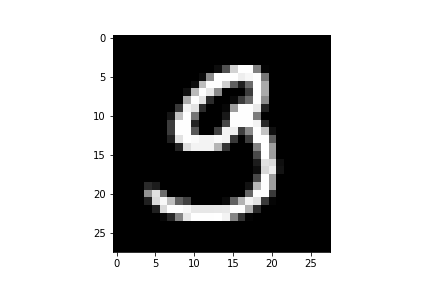
\includegraphics[scale=0.2]{Images/Graphics/MNIST/output0.png}
	
\includegraphics[scale=0.2]{Images/Graphics/MNIST/output1.png}
	
\includegraphics[scale=0.2]{Images/Graphics/MNIST/output2.png}
	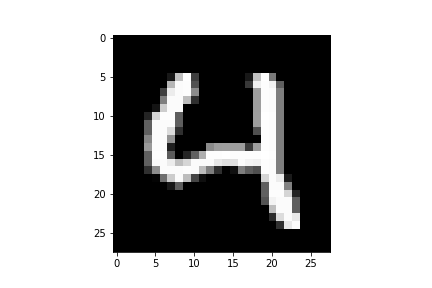
\includegraphics[scale=0.2]{Images/Graphics/MNIST/output3.png}
	
\includegraphics[scale=0.2]{Images/Graphics/MNIST/output4.png}
	
\includegraphics[scale=0.2]{Images/Graphics/MNIST/output5.png}
	
\includegraphics[scale=0.2]{Images/Graphics/MNIST/output6.png}
	
\includegraphics[scale=0.2]{Images/Graphics/MNIST/output7.png}
	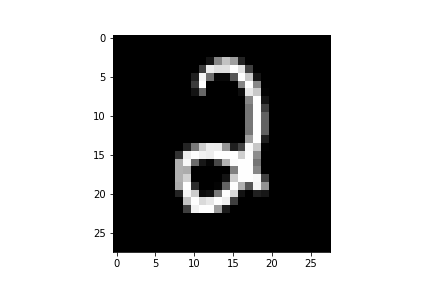
\includegraphics[scale=0.2]{Images/Graphics/MNIST/output8.png}
	
\includegraphics[scale=0.2]{Images/Graphics/MNIST/output9.png}
	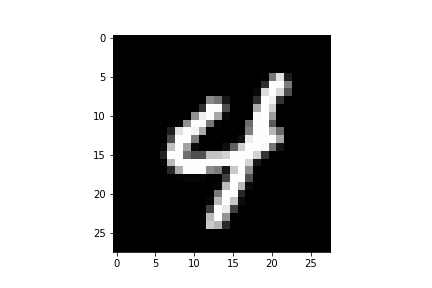
\includegraphics[scale=0.2]{Images/Graphics/MNIST/output10.png}
	
\includegraphics[scale=0.2]{Images/Graphics/MNIST/output11.png}
	
\includegraphics[scale=0.2]{Images/Graphics/MNIST/output12.png}
	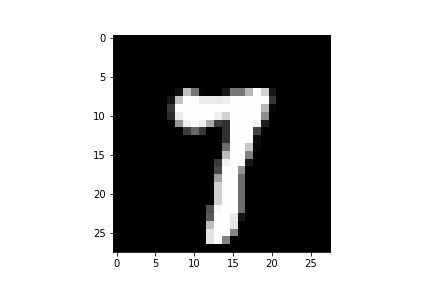
\includegraphics[scale=0.2]{Images/Graphics/MNIST/output13.png}
	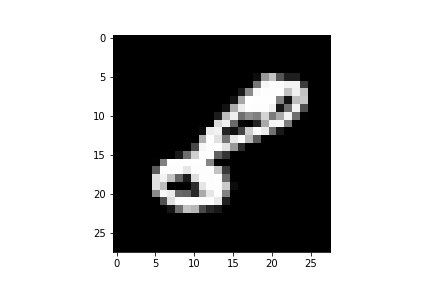
\includegraphics[scale=0.2]{Images/Graphics/MNIST/output14.png}
	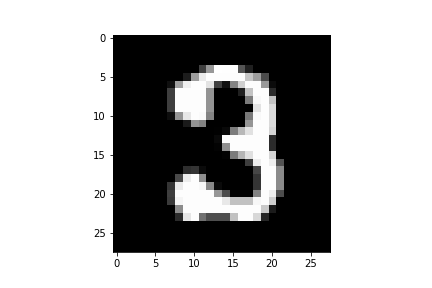
\includegraphics[scale=0.2]{Images/Graphics/MNIST/output15.png}
	
\includegraphics[scale=0.2]{Images/Graphics/MNIST/output16.png}
	
\includegraphics[scale=0.2]{Images/Graphics/MNIST/output17.png}
	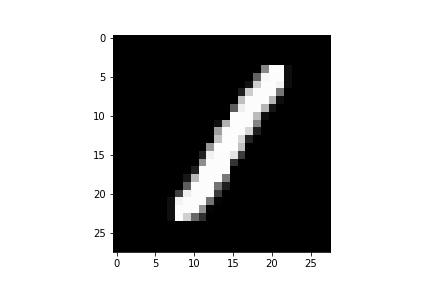
\includegraphics[scale=0.2]{Images/Graphics/MNIST/output18.png}
	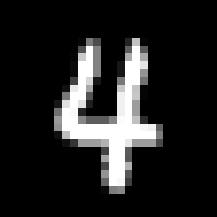
\includegraphics[scale=0.2]{Images/Graphics/MNIST/output19.png}
	
\includegraphics[scale=0.2]{Images/Graphics/MNIST/output20.png}
	
\includegraphics[scale=0.2]{Images/Graphics/MNIST/output21.png}
	
\includegraphics[scale=0.2]{Images/Graphics/MNIST/output22.png}
	
\includegraphics[scale=0.2]{Images/Graphics/MNIST/output23.png}
	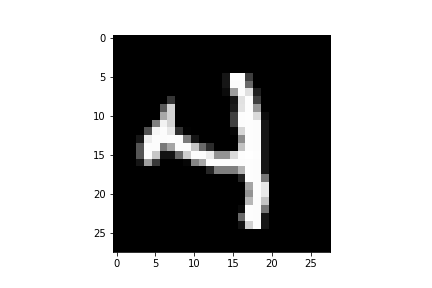
\includegraphics[scale=0.2]{Images/Graphics/MNIST/output24.png}
	
\includegraphics[scale=0.2]{Images/Graphics/MNIST/output25.png}
	
\includegraphics[scale=0.2]{Images/Graphics/MNIST/output26.png}
	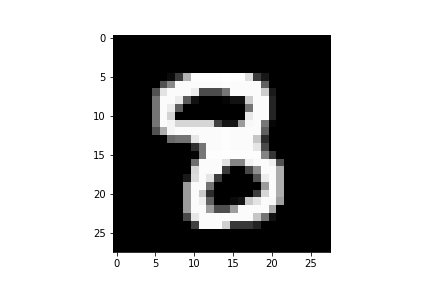
\includegraphics[scale=0.2]{Images/Graphics/MNIST/output27.png}
	
\includegraphics[scale=0.2]{Images/Graphics/MNIST/output28.png}
	
\includegraphics[scale=0.2]{Images/Graphics/MNIST/output29.png}
	\centering
	\caption{Datová sada MNIST}
\end{figure}

\section{Výsledky}

Přistupme nyní k samotnému srovnání algoritmů \emph{stochastický gradientní sestup},
\emph{metoda hybnosti} a~\emph{metoda Něstěrovovy hybnosti} (obě ve stochastické verzi).
Pro srovnání těchto algoritmů byly provedeny následující dva experimenty:
První se týká trénování jedné hluboké dopředné neuronové sítě těmito algoritmy pro úkol datové sady MNIST,
jež je uvedena výše v textu, a to konkrétně aplikací 5~000 iterací algoritmu
na nově inicializovanou síť.
Pro stochastický gradientní sestup byl použit řád učení o~hodnotě $10^{-2}$,
pro obě metody hybnosti byl použit řád učení $10^{-3}$ a koeficient $\alpha = 0.9$.
Dále uveďme velikost mini-dávky $M = 30$ pro všechny tři algoritmy.
V takovémto nastavení byly všechny tři algoritmy spuštěny stokrát.
Na výsledné distribuční funkce lze nahlédnout v obrázku (\ref{mlp_figure}).
Z grafu lze vyčíst takřka zanedbatelný rozdíl mezi metodou hybnosti a metodou Něstěrovovy hybnosti.
Dále graf vyjadřuje nemalou větší úspěšnost obyčejného stochastického gradientního sestupu.

Druhý experiment je téměř totožný, jen je použit jiný model neuronové sítě, a to konkrétně se zakomponovanou konvolucí.
Jinak je experiment totožný.
Proto lze z Obr. (\ref{cnn_figure}) odezřít výsledky, a to konkrétně, že stochastický gradientní sestup
má v tomto nastavení lepší výkonnost.

Pro srovnání algoritmů \emph{stochastický gradientní sestup}, \emph{AdaGrad}, \emph{RMSProp} a \emph{Adam}
lze využít podkladů na obrázku (\ref{mlp_advanced_figure}),
který zachycuje výsledky obdobných experimentů jako popsaných výše.
Nastavení tohoto pokusu bylo následující:
Pro stochastický gradientní sestup a algoritmus AdaGrad byl použit řád učení o hodnotě $10^{-2}$,
pro algoritmy RMSProp a Adam $10^{-3}$.
Pro AdaGrad bylo dále použito $\delta = 10^{-10}$,
pro RMSProp $\delta = 10^{-8}$ a $\rho = 0.99$,
pro Adam $\delta = 10^{-8}$, $\rho_1 = 0.9$ a $\rho_2 = 0.999$.
Úkol byl stejný - natrénovat tentýž model dopředné neuronové sítě pro klasifikaci číslic datové sady MNIST
za použití 5~000 iterací daného algoritmu.
Učení sítě vždy proběhlo stokrát.
Ze zmíněného obrázku vyplývá, že algoritmus AdaGrad je v tomto nastavení srovnatelný
se stochastickým gradientním sestupem
a že algoritmy RMSProp a Adam jsou minimálně pro toto specifické nastavení lepší.

Dále se pro srovnání algoritmů \emph{stochastický gradientní sestup}, \emph{AdaGrad}, \emph{RMSProp} a \emph{Adam}
lze opřít o výsledky vyobrazené na obrázku (\ref{cnn_advanced_figure}).
Ten zachycuje výsledky totožného nastavení jako obrázek (\ref{mlp_advanced_figure}) jen s rozdílem použitého modelu.
V tomto případě byl použit model konvoluční neuronové sítě.
Jak lze nahlédnout, algoritmus AdaGrad byl pro tuto úlohu nevhodný.
Algoritmus Adam dosáhl přijatelné úrovně neuronové sítě
(tedy úspěšnost na testovací datové sadě vyšší než 95~\%) zhruba v 60~\% případů,
algoritmus RMSProp zhruba v 90~\% případů
a stochastický gradientní sestup v 95~\% případů.
Ovšem kvalita přijatelně natrénovaných neuronových sítí byla v případě RMSProp vyšší
než u stochastického gradientního sestupu.

\begin{figure}
	\centering
	\begin{subfigure}[b]{0.45\textwidth}
		\centering
		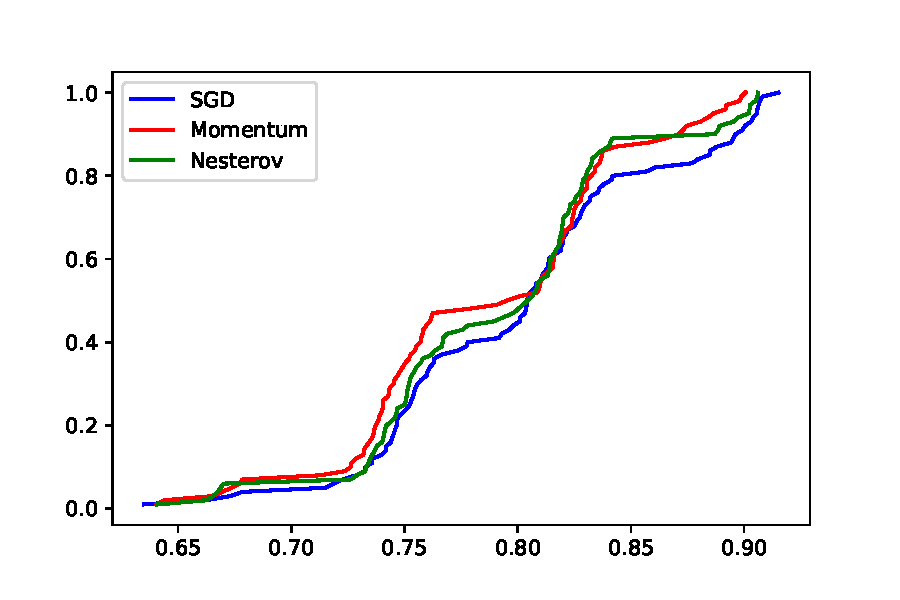
\includegraphics[width=\textwidth]{Images/Graphics/hubert.pdf}
		\caption{Srovnání algoritmů učení \Romannum{1}}
		\label{mlp_figure}
	\end{subfigure}
	\hfill
	\begin{subfigure}[b]{0.45\textwidth}
		\centering
		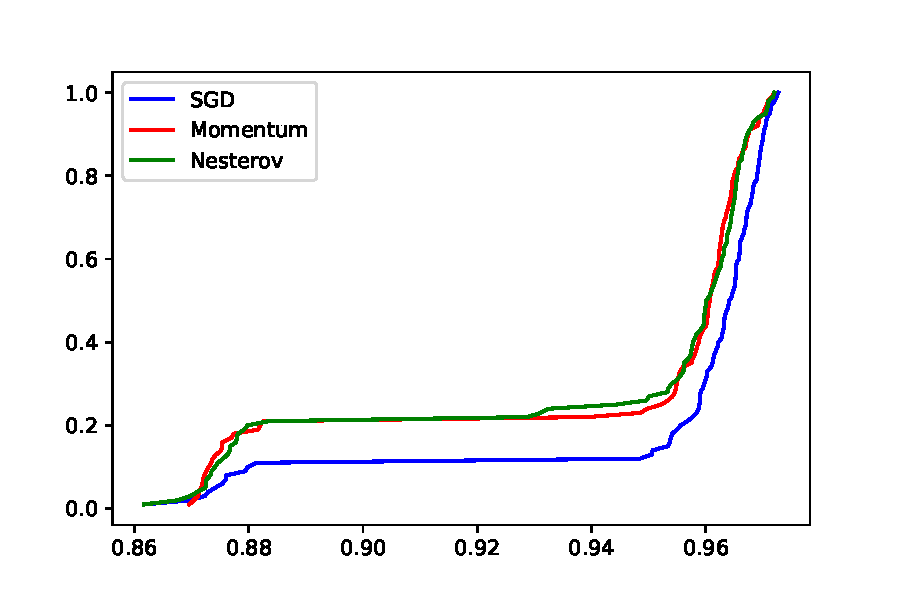
\includegraphics[width=\textwidth]{Images/Graphics/ivan.pdf}
		\caption{Srovnání algoritmů učení \Romannum{2}}
		\label{cnn_figure}
	\end{subfigure}

	\begin{subfigure}[b]{0.45\textwidth}
		\centering
		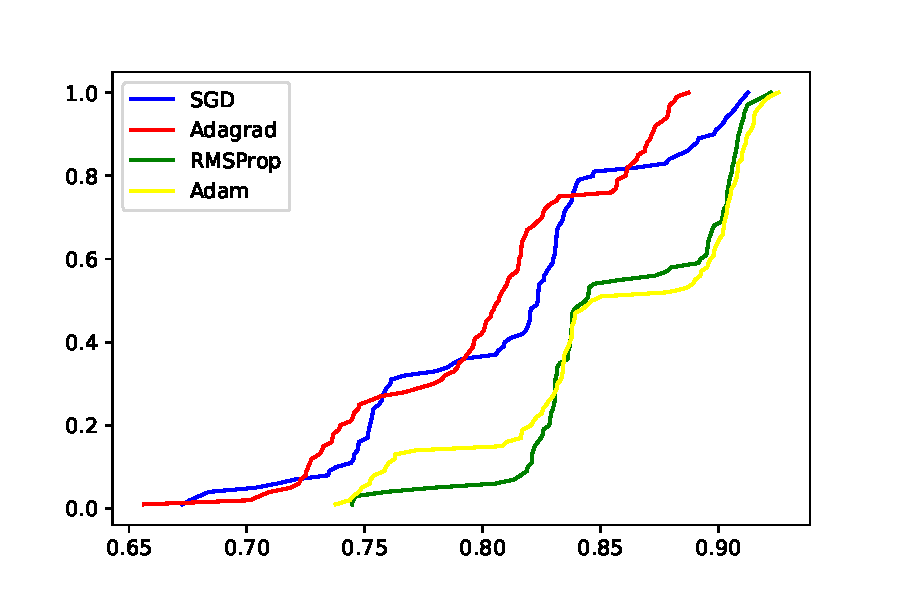
\includegraphics[width=\textwidth]{Images/Graphics/nevil.pdf}
		\caption{Srovnání algoritmů učení \Romannum{3}}
		\label{mlp_advanced_figure}
	\end{subfigure}
	\hfill
	\begin{subfigure}[b]{0.45\textwidth}
		\centering
		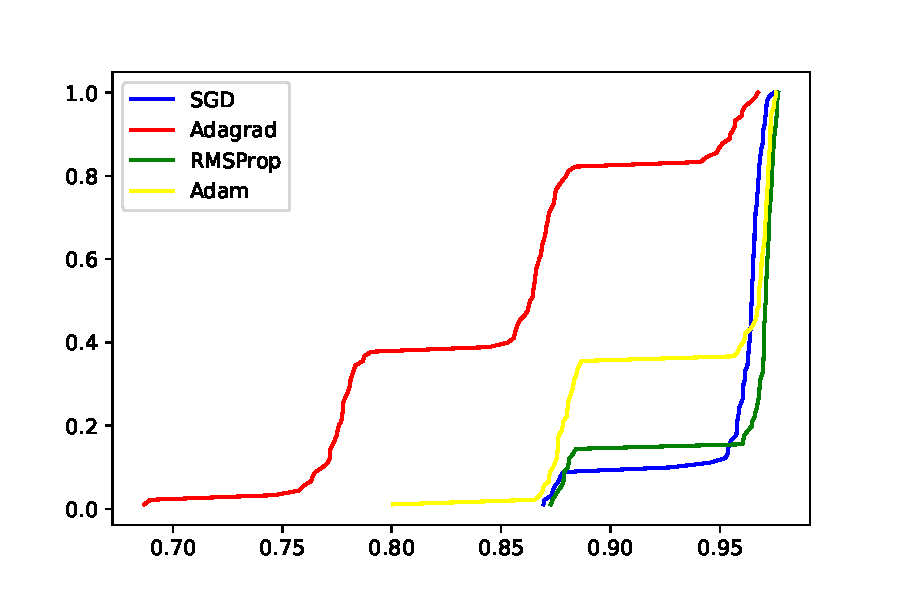
\includegraphics[width=\textwidth]{Images/Graphics/oto.pdf}
		\caption{Srovnání algoritmů učení \Romannum{4}}
		\label{cnn_advanced_figure}
	\end{subfigure}
	\caption{Srovnání algoritmů učení}
	\emph{SGD} - stochastický gradientní sestup;
	\emph{Momentum} - metoda hybnosti;
	\emph{Nesterov} - metoda Něstěrovovy hybnosti;
	\emph{AdaGrad} - algoritmus AdaGrad;
	\emph{RMSProp} - algoritmus RMSProp;
	\emph{Adam} - algoritmus Adam.
\end{figure}

\chapter{Vygenerované adversariální vzorky}

\section{Srovnání metod}
% Mega obrázek, kvalitativní srovnání, úspěšnost útoků, vše v L^\infty normě

Přistupme nyní ke srovnání účinnosti metod generování adversariálních vzorků,
které byly představeny výše, totiž metod \emph{FGSM}, \emph{I-FGSM}, \emph{PGD}, \emph{cílená optimalizační úloha}
a \emph{CW}.

\subsection{Klasifikační úkol}

Úkol, na kterém budeme metody srovnávat je tentýž jako v případě srovnání algoritmů učení.
Jedná se tedy o problém klasifikace ručně psaných číslic datové sady MNIST \cite{MNIST}.
Cílem metod bude tedy vytvořit perturbovaný obrázek číslice stejných rozměrů jako jsou obrázky oné datové sady s tím,
že snahou bude vytvořit takovou perturbaci,
pro kterou dojde po jejím přičtení k obrázku z datové sady k nesprávné klasifikaci.

\subsection{Použitý model}

Jelikož všechny tyto metody pracují na \emph{white-box} principu,
je nutné k jejich provedení mít k dispozici natrénovanou klasifikační neuronovou síť.
Za tuto je zvolen model konvoluční neuronové sítě složené po řadě z vrstev:
\begin{enumerate} \setlength{\itemsep}{-5pt}
	\item Konvoluční vrstva s $1$ vstupním kanálem, $32$ výstupními kanály a jádrem konvoluce $3 \times 3$,
	% \itemsep{0cm}
	\item aktivační vrstva s funkcí ReLU,
	\item konvoluční vrstva s $32$ vstupními kanály, $32$ výstupními kanály a jádrem konvoluce $3 \times 3$,
	\item aktivační vrstva s funkcí ReLU,
	\item max pooling vrstva s rozměry jádra $2 \times 2$,
	\item konvoluční vrstva s $32$ vstupními kanály, $64$ výstupními kanály a jádrem konvoluce $3 \times 3$,
	\item aktivační vrstva s funkcí ReLU,
	\item konvoluční vrstva s $64$ vstupními kanály, $64$ výstupními kanály a jádrem konvoluce $3 \times 3$,
	\item aktivační vrstva s funkcí ReLU,
	\item max pooling vrstva s rozměry jádra $2 \times 2$,
	\item hustá vrstva s $1024$ vstupy a $200$ výstupy,
	\item aktivační vrstva s funkcí ReLU,
	\item hustá vrstva s $200$ vstupy a $10$ výstupy,
	\item aktivační vrstva s funkcí softmax.
\end{enumerate}

Tento model byl trénován pomocí algoritmu RMSProp s řádem učení $\epsilon = 10^{-3}$,
decay rate $\rho = 0.99$ a stabilizační konstantou $\delta = 10^{-8}$.
Použito bylo $3250$ iterací tohoto algoritmu
a bylo dosaženo úspěšnosti $97.57 \%$ na testovací datové sadě.

\subsection{Norma perturbace}

Pro srovnání metod generování adversariálních vzorků byla zvolena
\emph{maximová}, tedy \emph{$l_\infty$} norma.
Za toleranci v této normě, resp. velikost perturbace byl zvolen ekvivalent
$50$ pixelových bodů, to jest $\kappa = \frac{50}{255}$,
jelikož hodnoty pixelů obrázku jsou lineárně přeškálovány do intervalu $[0, 1]$.

Připomeňme, kde figuruje volba normy v předpisech jednotlivých metod generování adversariálních vzorků.
Pro FGSM útok se volba $l_\infty$ normy odráží v tom,
že se k benignímu obrázku přičítá $\kappa$ násobek znaménka gradientu,
tedy z tohoto je nutně norma perturbace $\|\Delta x\|_\infty = \kappa$
a je možné splnit definici adversariálního vzorku.
Pro I-FGSM a PGD se volba normy odráží ve funkci \emph{Clip},
která zajišťuje, že norma perturbace $\|\Delta x\|_\infty \leq \kappa$.
Pro cílenou optimalizační úlohu a CW útok je volba normy důležitá jednak
pro množinu kde minimum z příslušné funkce hledáme,
a jednak pro samotnou funkci, jejíž minimum metoda hledá.

\subsection{Implementační detaily}

Metoda FGSM byla implementována podle předpisu uvedeném v předchozích kapitolách.

Pro metody I-FGSM a PGD byl zvolen krok algoritmu $\gamma = 10^{-2}$
a počet iterací $62$ podle návrhu v~\cite{I_FGSM}.

Cílená optimalizační byla implementována algoritmem sign gradient descent,
s krokem $10^{-2}$ a $100$ iteracemi, kde parametr $\lambda$ byl volen nejprve jako $\lambda = 10^{-2}$
a při neúspěchu nahrazen dle pravidla
\begin{equation}
	\lambda \leftarrow 10 \cdot \lambda.
\end{equation}
Pro $\lambda \geq 100$ pak metoda vrátila poslední nalezený, byť stále správně klasifikovaný, vzorek.
Takto jednoduše byl line-search algoritmus implementován z důvodu výpočetní náročnosti složitějších implementací algoritmu.
Tato procedura byla aplikována pro všechny možné cílové značky
a za výsledný vzorek položila ten nejbližší (ve smyslu $l_\infty$ normy)
původnímu benignímu vzorku z těch, které byly nesprávně klasifikovány.

Metoda CW byla implementována obdobně jako cílená optimalizační metoda
pomocí sign gradient descentu s krokem $10^{-2}$ a $100$ iteracemi.
Parametr $\lambda$ byl zvolen pevně jako $\lambda = 1$.

\subsection{Výsledky}

Bylo provedeno generování adversariálních vzorků všemi těmito metodami
a za benigní vzorky bylo použito $1000$ vzorků trénovací datové sady MNIST.
Za úspěšnost metody uvažme procentuální podíl špatně klasifikovaných adversariálních vzorků.
Potom lze uvést dle tabulky \ref{allgen_success},
že nejúspěšnější metodou v tomto nastavení je cílená optimalizační metoda.
Nejméně úspěšnou metodou v tomto nastavení je naopak FGSM.

\begin{table}
	\centering
	\begin{tabular}{| c | c |}
		\hline
		Metoda & Úspěšnost \\
		\hline
		FGSM & 40.4 \% \\
		I-FGSM & 78.4 \% \\
		PGD & 78.8 \% \\
		Cílená optimalizační metoda & 100 \% \\
		CW & 99.7 \% \\
		\hline
	\end{tabular}
	\caption{Úspěšnost metod generování adversariálních vzorků}
	\label{allgen_success}
\end{table}

Na příklady vzorků vygenerovaných výše uvedenými metodami lze nahlédnout v obrázku \ref{allgen}.
Jak je vidět, všechny metody při výše popsané volbě parametrů a implementačních detailů
přidávají benigním vzorkům do pozadí jakési artefakty.
U vzorků vygenerovaných metodou CW ovšem dochází k nadměrnému zkreslení.
Je to dáno nesprávnou volbou parametru $\lambda$.
Diskuze ohledně tohoto typu útoku následuje v další sekci textu.

\begin{figure}
	\begin{subfigure}[b]{\textwidth}
		
\includegraphics[width=0.09\textwidth]{Images/Graphics/AEXAMPLES/ALLGEN/benign_1.png}
		
\includegraphics[width=0.09\textwidth]{Images/Graphics/AEXAMPLES/ALLGEN/benign_3.png}
		
\includegraphics[width=0.09\textwidth]{Images/Graphics/AEXAMPLES/ALLGEN/benign_5.png}
		
\includegraphics[width=0.09\textwidth]{Images/Graphics/AEXAMPLES/ALLGEN/benign_7.png}
		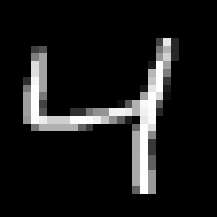
\includegraphics[width=0.09\textwidth]{Images/Graphics/AEXAMPLES/ALLGEN/benign_2.png}
		
\includegraphics[width=0.09\textwidth]{Images/Graphics/AEXAMPLES/ALLGEN/benign_34.png}
		
\includegraphics[width=0.09\textwidth]{Images/Graphics/AEXAMPLES/ALLGEN/benign_18.png}
		
\includegraphics[width=0.09\textwidth]{Images/Graphics/AEXAMPLES/ALLGEN/benign_37.png}
		
\includegraphics[width=0.09\textwidth]{Images/Graphics/AEXAMPLES/ALLGEN/benign_17.png}
		
\includegraphics[width=0.09\textwidth]{Images/Graphics/AEXAMPLES/ALLGEN/benign_4.png}
		\centering
		\caption{Benigní vzorky}
	\end{subfigure}
	\begin{subfigure}[b]{\textwidth}
		
\includegraphics[width=0.09\textwidth]{Images/Graphics/AEXAMPLES/ALLGEN/fgsm_1.png}
		
\includegraphics[width=0.09\textwidth]{Images/Graphics/AEXAMPLES/ALLGEN/fgsm_3.png}
		
\includegraphics[width=0.09\textwidth]{Images/Graphics/AEXAMPLES/ALLGEN/fgsm_5.png}
		
\includegraphics[width=0.09\textwidth]{Images/Graphics/AEXAMPLES/ALLGEN/fgsm_7.png}
		\includegraphics[width=0.09\textwidth]{Images/Graphics/AEXAMPLES/ALLGEN/fgsm_2.png}
		\includegraphics[width=0.09\textwidth]{Images/Graphics/AEXAMPLES/ALLGEN/fgsm_34.png}
		\includegraphics[width=0.09\textwidth]{Images/Graphics/AEXAMPLES/ALLGEN/fgsm_18.png}
		\includegraphics[width=0.09\textwidth]{Images/Graphics/AEXAMPLES/ALLGEN/fgsm_37.png}
		\includegraphics[width=0.09\textwidth]{Images/Graphics/AEXAMPLES/ALLGEN/fgsm_17.png}
		\includegraphics[width=0.09\textwidth]{Images/Graphics/AEXAMPLES/ALLGEN/fgsm_4.png}
		\centering
		\caption{FGSM}
	\end{subfigure}
	\begin{subfigure}[b]{\textwidth}
		\includegraphics[width=0.09\textwidth]{Images/Graphics/AEXAMPLES/ALLGEN/ifgsm_1.png}
		\includegraphics[width=0.09\textwidth]{Images/Graphics/AEXAMPLES/ALLGEN/ifgsm_3.png}
		\includegraphics[width=0.09\textwidth]{Images/Graphics/AEXAMPLES/ALLGEN/ifgsm_5.png}
		\includegraphics[width=0.09\textwidth]{Images/Graphics/AEXAMPLES/ALLGEN/ifgsm_7.png}
		\includegraphics[width=0.09\textwidth]{Images/Graphics/AEXAMPLES/ALLGEN/ifgsm_2.png}
		\includegraphics[width=0.09\textwidth]{Images/Graphics/AEXAMPLES/ALLGEN/ifgsm_34.png}
		\includegraphics[width=0.09\textwidth]{Images/Graphics/AEXAMPLES/ALLGEN/ifgsm_18.png}
		\includegraphics[width=0.09\textwidth]{Images/Graphics/AEXAMPLES/ALLGEN/ifgsm_37.png}
		\includegraphics[width=0.09\textwidth]{Images/Graphics/AEXAMPLES/ALLGEN/ifgsm_17.png}
		\includegraphics[width=0.09\textwidth]{Images/Graphics/AEXAMPLES/ALLGEN/ifgsm_4.png}
		\centering
		\caption{I-FGSM}
	\end{subfigure}
	\begin{subfigure}[b]{\textwidth}
		\includegraphics[width=0.09\textwidth]{Images/Graphics/AEXAMPLES/ALLGEN/pgd_1.png}
		\includegraphics[width=0.09\textwidth]{Images/Graphics/AEXAMPLES/ALLGEN/pgd_3.png}
		\includegraphics[width=0.09\textwidth]{Images/Graphics/AEXAMPLES/ALLGEN/pgd_5.png}
		\includegraphics[width=0.09\textwidth]{Images/Graphics/AEXAMPLES/ALLGEN/pgd_7.png}
		\includegraphics[width=0.09\textwidth]{Images/Graphics/AEXAMPLES/ALLGEN/pgd_2.png}
		\includegraphics[width=0.09\textwidth]{Images/Graphics/AEXAMPLES/ALLGEN/pgd_34.png}
		\includegraphics[width=0.09\textwidth]{Images/Graphics/AEXAMPLES/ALLGEN/pgd_18.png}
		\includegraphics[width=0.09\textwidth]{Images/Graphics/AEXAMPLES/ALLGEN/pgd_37.png}
		\includegraphics[width=0.09\textwidth]{Images/Graphics/AEXAMPLES/ALLGEN/pgd_17.png}
		\includegraphics[width=0.09\textwidth]{Images/Graphics/AEXAMPLES/ALLGEN/pgd_4.png}
		\centering
		\caption{PGD}
	\end{subfigure}
	\begin{subfigure}[b]{\textwidth}
		\includegraphics[width=0.09\textwidth]{Images/Graphics/AEXAMPLES/ALLGEN/lbfgs_1.png}
		\includegraphics[width=0.09\textwidth]{Images/Graphics/AEXAMPLES/ALLGEN/lbfgs_3.png}
		\includegraphics[width=0.09\textwidth]{Images/Graphics/AEXAMPLES/ALLGEN/lbfgs_5.png}
		\includegraphics[width=0.09\textwidth]{Images/Graphics/AEXAMPLES/ALLGEN/lbfgs_7.png}
		\includegraphics[width=0.09\textwidth]{Images/Graphics/AEXAMPLES/ALLGEN/lbfgs_2.png}
		\includegraphics[width=0.09\textwidth]{Images/Graphics/AEXAMPLES/ALLGEN/lbfgs_34.png}
		\includegraphics[width=0.09\textwidth]{Images/Graphics/AEXAMPLES/ALLGEN/lbfgs_18.png}
		\includegraphics[width=0.09\textwidth]{Images/Graphics/AEXAMPLES/ALLGEN/lbfgs_37.png}
		\includegraphics[width=0.09\textwidth]{Images/Graphics/AEXAMPLES/ALLGEN/lbfgs_17.png}
		\includegraphics[width=0.09\textwidth]{Images/Graphics/AEXAMPLES/ALLGEN/lbfgs_4.png}
		\centering
		\caption{Cílená optimalizační metoda}
	\end{subfigure}
	\begin{subfigure}[b]{\textwidth}
		\includegraphics[width=0.09\textwidth]{Images/Graphics/AEXAMPLES/ALLGEN/cw_1.png}
		\includegraphics[width=0.09\textwidth]{Images/Graphics/AEXAMPLES/ALLGEN/cw_3.png}
		\includegraphics[width=0.09\textwidth]{Images/Graphics/AEXAMPLES/ALLGEN/cw_5.png}
		\includegraphics[width=0.09\textwidth]{Images/Graphics/AEXAMPLES/ALLGEN/cw_7.png}
		\includegraphics[width=0.09\textwidth]{Images/Graphics/AEXAMPLES/ALLGEN/cw_2.png}
		\includegraphics[width=0.09\textwidth]{Images/Graphics/AEXAMPLES/ALLGEN/cw_34.png}
		\includegraphics[width=0.09\textwidth]{Images/Graphics/AEXAMPLES/ALLGEN/cw_18.png}
		\includegraphics[width=0.09\textwidth]{Images/Graphics/AEXAMPLES/ALLGEN/cw_37.png}
		\includegraphics[width=0.09\textwidth]{Images/Graphics/AEXAMPLES/ALLGEN/cw_17.png}
		\includegraphics[width=0.09\textwidth]{Images/Graphics/AEXAMPLES/ALLGEN/cw_4.png}
		\centering
		\caption{CW}
	\end{subfigure}
	\centering
	\caption{Vzorky generované různými metodami hledání adversariálních vzorků}
	\label{allgen}
\end{figure}

% \section{Metody založené na FGSM}

% \section{Analýza cílené optimalizační metody}
% % Srovnání best case a worst case, resp. cross-label tabulka

\section{Analýza CW útoku}
% Variabilita v parametru c a volba normy
% Při jakém c mi to fliplo? Odkázat na best case L-BFGS

Podívejme se nyní na samotnou metodu CW útoku.
V předcházející části textu došlo k pevnému výběru $l_p$ normy, která figuruje v předpisu metody,
a parametru $\lambda$.
Zkusme proto zjistit, jaký vliv tyto volby mají na úspěšnost útoku a na kvalitu nalezených vzorků.

\subsection{Vliv volby parametru $\lambda$}

Z předpisu pro CW metodu lze odvodit, že větší hodnota $\lambda$ napomáhá adversarialitě vzorku,
tak jinak je spíše špatně klasifikován, než při volbě menší hodnoty $\lambda$.
Je to ovšem za cenu vyšší vzdálenosti (ve smyslu použité $l_p$ normy) nalezeného vzorku od původního benigního vzorku,
tedy dojde k většímu zkreslení vzorku.
Jak lze vyčíst z tabulky \ref{cw_success} a odvodit z obrázků \ref{cw_images_four} a \ref{cw_images_eight},
tato úvaha je správná.

\subsection{Vliv volby normy}

Za normy byly v provedených numerických experimentech dosazeny $l_\infty$, $l_1$ a $l_2$ normy.
Jak lze nahlédnout v obrázcích \ref{cw_images_four} a \ref{cw_images_eight},
použití $l_\infty$ normy vede k silnému zkreslení.
Je to dáno faktem, že tato norma při derivování, které se používá pro numerické optimalizační algoritmy,
vyzdvihne pouze jeden pixel obrázku, zbylé nechává netknuté.
Použití $l_1$ či $l_2$ normy potom vede ke kultivovanějším obrázkům.
Tím je myšleno, že vzniklé obrázky pozbývají náhodně vypadající artefakty v pozadí číslice.

\begin{table}
	\centering
	\begin{tabular}{| c || c | c | c | c |}
		\hline
		Algoritmus & $\lambda$ & & & \\
		\hline
		Norma & 0.1 & 1 & 10 & 100 \\
		\hline
		\hline
		$l_\infty$ & 99.6 \% & 99.7 \% & 99.8 \% & 99.8 \% \\
		\hline
		$l_1$ & 0 \% & 32.5 \% & 88.9 \% & 91.7 \% \\
		\hline
		$l_2$ & 23.9 \% & 93.6 \% & 100 \% & 100 \% \\
		\hline
	\end{tabular}
	\caption{Úspěšnost CW útoku v závislosti na zvolených parametrech}
	\label{cw_success}
\end{table}

\begin{figure}
	\centering
	\begin{subfigure}[b]{\textwidth}
		\centering
		\includegraphics[width=0.1\textwidth]{Images/Graphics/AEXAMPLES/CW_BATCH_NOCLIP/benign_2.png}
		\caption{Benigní vzorek}
	\end{subfigure}
	\begin{subfigure}[b]{\textwidth}
		\centering
		\includegraphics[width=0.1\textwidth]{Images/Graphics/AEXAMPLES/CW_BATCH_NOCLIP/c_lambda_0.1_cw_linfty_2.png}
		\includegraphics[width=0.1\textwidth]{Images/Graphics/AEXAMPLES/CW_BATCH_NOCLIP/c_lambda_1_cw_linfty_2.png}
		\includegraphics[width=0.1\textwidth]{Images/Graphics/AEXAMPLES/CW_BATCH_NOCLIP/c_lambda_10_cw_linfty_2.png}
		\includegraphics[width=0.1\textwidth]{Images/Graphics/AEXAMPLES/CW_BATCH_NOCLIP/c_lambda_100_cw_linfty_2.png}
		\caption{$l_\infty$ útok}
	\end{subfigure}
	\begin{subfigure}[b]{\textwidth}
		\centering
		\includegraphics[width=0.1\textwidth]{Images/Graphics/AEXAMPLES/CW_BATCH_NOCLIP/c_lambda_0.1_cw_lone_2.png}
		\includegraphics[width=0.1\textwidth]{Images/Graphics/AEXAMPLES/CW_BATCH_NOCLIP/c_lambda_1_cw_lone_2.png}
		\includegraphics[width=0.1\textwidth]{Images/Graphics/AEXAMPLES/CW_BATCH_NOCLIP/c_lambda_10_cw_lone_2.png}
		\includegraphics[width=0.1\textwidth]{Images/Graphics/AEXAMPLES/CW_BATCH_NOCLIP/c_lambda_100_cw_lone_2.png}
		\caption{$l_1$ útok}
	\end{subfigure}
	\begin{subfigure}[b]{\textwidth}
		\centering
		\includegraphics[width=0.1\textwidth]{Images/Graphics/AEXAMPLES/CW_BATCH_NOCLIP/c_lambda_0.1_cw_ltwo_2.png}
		\includegraphics[width=0.1\textwidth]{Images/Graphics/AEXAMPLES/CW_BATCH_NOCLIP/c_lambda_1_cw_ltwo_2.png}
		\includegraphics[width=0.1\textwidth]{Images/Graphics/AEXAMPLES/CW_BATCH_NOCLIP/c_lambda_10_cw_ltwo_2.png}
		\includegraphics[width=0.1\textwidth]{Images/Graphics/AEXAMPLES/CW_BATCH_NOCLIP/c_lambda_100_cw_ltwo_2.png}
		\caption{$l_2$ útok}
	\end{subfigure}
	\caption{Výsledky CW útoku pro různé volby parametrů; $\lambda$ je voleno po řadě $0.1$, $1$, $10$ a $100$}
	\label{cw_images_four}
\end{figure}

\begin{figure}
	\centering
	\begin{subfigure}[b]{\textwidth}
		\centering
		\includegraphics[width=0.1\textwidth]{Images/Graphics/AEXAMPLES/CW_BATCH_NOCLIP/benign_17.png}
		\caption{Benigní vzorek}
	\end{subfigure}
	\begin{subfigure}[b]{\textwidth}
		\centering
		\includegraphics[width=0.1\textwidth]{Images/Graphics/AEXAMPLES/CW_BATCH_NOCLIP/c_lambda_0.1_cw_linfty_17.png}
		\includegraphics[width=0.1\textwidth]{Images/Graphics/AEXAMPLES/CW_BATCH_NOCLIP/c_lambda_1_cw_linfty_17.png}
		\includegraphics[width=0.1\textwidth]{Images/Graphics/AEXAMPLES/CW_BATCH_NOCLIP/c_lambda_10_cw_linfty_17.png}
		\includegraphics[width=0.1\textwidth]{Images/Graphics/AEXAMPLES/CW_BATCH_NOCLIP/c_lambda_100_cw_linfty_17.png}
		\caption{$l_\infty$ útok}
	\end{subfigure}
	\begin{subfigure}[b]{\textwidth}
		\centering
		\includegraphics[width=0.1\textwidth]{Images/Graphics/AEXAMPLES/CW_BATCH_NOCLIP/c_lambda_0.1_cw_lone_17.png}
		\includegraphics[width=0.1\textwidth]{Images/Graphics/AEXAMPLES/CW_BATCH_NOCLIP/c_lambda_1_cw_lone_17.png}
		\includegraphics[width=0.1\textwidth]{Images/Graphics/AEXAMPLES/CW_BATCH_NOCLIP/c_lambda_10_cw_lone_17.png}
		\includegraphics[width=0.1\textwidth]{Images/Graphics/AEXAMPLES/CW_BATCH_NOCLIP/c_lambda_100_cw_lone_17.png}
		\caption{$l_1$ útok}
	\end{subfigure}
	\begin{subfigure}[b]{\textwidth}
		\centering
		\includegraphics[width=0.1\textwidth]{Images/Graphics/AEXAMPLES/CW_BATCH_NOCLIP/c_lambda_0.1_cw_ltwo_17.png}
		\includegraphics[width=0.1\textwidth]{Images/Graphics/AEXAMPLES/CW_BATCH_NOCLIP/c_lambda_1_cw_ltwo_17.png}
		\includegraphics[width=0.1\textwidth]{Images/Graphics/AEXAMPLES/CW_BATCH_NOCLIP/c_lambda_10_cw_ltwo_17.png}
		\includegraphics[width=0.1\textwidth]{Images/Graphics/AEXAMPLES/CW_BATCH_NOCLIP/c_lambda_100_cw_ltwo_17.png}
		\caption{$l_2$ útok}
	\end{subfigure}
	\caption{Výsledky CW útoku pro různé volby parametrů; $\lambda$ je voleno po řadě $0.1$, $1$, $10$ a $100$}
	\label{cw_images_eight}
\end{figure}

% Při hlubším studiu CW útoku lze dojít k několika závěrům.
% Jeden se týká volby použité $l_{p}$ normy, další detailu implementace,
% totiž jestli dojde k aplikaci funkce Clip \emph{vždy} při každé iteraci algoritmu sign gradient descent,
% nebo \emph{jednou} na konci procesu generování adversariálních vzorků.
% A v neposlední řadě lze zkoumat vliv parametru $\lambda$ na úspěšnost metody.

% \subsection{Vliv volby normy na parametr $\kappa$}

% Parametrem $\kappa$ myslíme poloměr kulového okolí benigního vzorku v příslušné $l_p$ normě,
% kde hledáme adversariální vzorek.
% V předcházející sekci bylo zvoleno pevně $\kappa = \frac{50}{255}$ pro $l_\infty$ normu.
% To umožňuje každé složce vzorku změnit svou hodnotu o $50$ pixelových bodů.

% Použijeme-li ovšem stejné $\kappa$ pro $l_1$ normu,
% dovolíme jen jedné složce vzorku změnit svou hodnotu o $50$ pixelových bodů
% nebo dvěma složkám o $25$ pixelových bodů atp.
% Z této úvahy je zřejmé, že se změnou normy musí nastat i změna $\kappa$.

% Označme proto ono pevně zvolené $\kappa$ pro $l_\infty$ normu jako $\kappa_\infty$
% a odvoďme, jak by mělo vypadat $\kappa_1$ pro $l_1$ normu a $\kappa_2$ pro $l_2$ normu,
% abychom dovolili v zásadě stejnou změnu hodnot složek vzorku.

% Pro vektor $u$ dimenze $k$ platí:
% \begin{align}
% 	\|u\|_1 &= \sum_{i=1}^k \left|u_i\right| < \sum_{i=1}^k \operatorname{max}_{i = 1, ..., k} \left|u_i\right| = k \cdot \|u\|_\infty, \\
% 	\|u\|_2^2 &= \sum_{i=1}^k \left|u_i\right|^2 < \sum_{i=1}^k \operatorname{max}_{i = 1, ..., k} \left|u_i\right|^2 = k \cdot \|u\|_\infty^2.
% \end{align}
% Odtud lze s přihlédnutím k faktu, že pro náš úkol užíváme vzorky o velikosti $28 \times 28$,
% volit: 
% \begin{align}
% 	\kappa_1 &= 28 \cdot 28 \cdot \kappa_\infty, \\
% 	\kappa_2 &= \sqrt{28 \cdot 28} \cdot \kappa_\infty = 28 \cdot \kappa_\infty.
% \end{align}

% \subsection{Výsledky}

% Byly implementovány útoky s použitím $l_\infty$, $l_1$ a $l_2$ normy
% vždy ve dvou verzích, jedna, kdy je funkce Clip aplikována vždy,
% a druhá, kdy je funkce Clip aplikována jednou.
% Následně byl pomocí každé z těchto implementací proveden útok na $100$ vzorcích trénovací sady MNIST
% pro různé volby parametru $\lambda$.
% Konkrétně po řadě pro hodnoty $\lambda$ $0.1$, $1$, $10$ a $100$.
% Na úspěšnost jednotlivých útoků lze nahlédnout v tabulce \ref{cw_success}
% a na příklad vygenerovaných adversariálních vzorků v obrázku \ref{cw_images}.

% Tyto výsledky dávají podnět k vyslovení následujících pozorování.
% $l_\infty$ útok je uspěšný pouze pro verzi, kdy je funkce Clip aplikována vždy.
% Navíc tento útok vykazuje při této implementaci invarianci vůči volbě hodnoty parametru $\lambda$.
% % TODO: Vysvětlení
% Úspěšnost $l_1$ útoku je srovnatelná v nastavení, kdy je funkce Clip aplikována vždy,
% s nastavením, kdy je funkce Clip aplikována jednou.
% Oproti $l_\infty$ útoku ovšem vykazuje silnou závislost na volbě hodnoty parametru $\lambda$,
% kdy metoda je úspěšnější pro vyšší hodnoty $\lambda$.
% CW útok využívající normu $l_2$ je jako $l_\infty$ útok závislý na implementaci,
% zda je funkce Clip aplikována vždy, nebo jednou,
% avšak v případě $l_2$ normy je závislost opačná,
% totiž $l_2$ útok je úspěšný v nastavení \emph{jednou}
% a v nastavení \emph{vždy} nemá zdaleka takovou úspěšnost.
% Stejně jako $l_1$ útok je $l_2$ útok závislý na volbě hodnoty parametru $\lambda$,
% a to tak, že větší hodnota $\lambda$ poskytuje větší úspěšnost útoku.
% Celkově je $l_2$ CW útok při vhodném nastavení parametrů v této implementaci
% nejúspěšnější metoda generování adversariálních vzorků ze všech zkoumaných metod,
% jelikož dosahuje úspěšnosti $94 \%$.

% Další pozorování se týká samotné podoby jednotlivých útoků.
% Zatímco $l_\infty$ útok přidává podobně jako metody založené na FGSM útoku
% jakési artefakty do pozadí obrázku,
% $l_1$ útok se zaměřuje pouze na samotnou číslici, a to zatmavením některých pixelů číslice.
% U $l_2$ útoku si lze všimnout kombinace předchozího.
% $l_2$ útok jednak zatmavuje vybrané pixely číslice, jednak přidává artefakty do pozadí číslice.
% Jak je patrné z obrázku \ref{cw_ltwo},
% tyto artefakty se ovšem jako v případě $l_\infty$ útoku nezdají být náhodné.
% $l_2$ útok v tomto konkrétním případě dokreslil do obrázku číslice jedna vodorovnou čáru v místě,
% kde se obvykle nachází vodorovná čára číslice sedm.


% \begin{table}
% 	\centering
% 	\begin{tabular}{| c | c || c | c | c | c |}
% 		\hline
% 		Algoritmus & & $\lambda$ & & & \\
% 		\hline
% 		Norma & Clip & 0.1 & 1 & 10 & 100 \\
% 		\hline
% 		\hline
% 		$l_\infty$ & Vždy & 74 \% & 74 \% & 74 \% & 74 \% \\
% 		\hline
% 		$l_1$ & Vždy & 0 \% & 50 \% & 87 \% & 90 \% \\
% 		\hline
% 		$l_2$ & Vždy & 1 \% & 8 \% & 14 \% & 16 \% \\
% 		\hline
% 		$l_\infty$ & Jednou & 0 \% & 0 \% & 0 \% & 0 \% \\
% 		\hline
% 		$l_1$ & Jednou & 0 \% & 33 \% & 89 \% & 93 \% \\
% 		\hline
% 		$l_2$ & Jednou & 8 \% & 87 \% & 94 \% & 94 \% \\
% 		\hline
% 	\end{tabular}
% 	\caption{Úspěšnost CW útoku v závislosti na zvolených parametrech}
% 	\label{cw_success}
% \end{table}

% \begin{figure}
% 	\centering
% 	\begin{subfigure}[b]{\textwidth}
% 		\centering
% 		\includegraphics[width=0.1\textwidth]{Images/Graphics/AEXAMPLES/CW_BATCH/benign_2.png}
% 		\caption{Benigní vzorek}
% 	\end{subfigure}
% 	\begin{subfigure}[b]{\textwidth}
% 		\centering
% 		\includegraphics[width=0.1\textwidth]{Images/Graphics/AEXAMPLES/CW_BATCH/clip_always_c_lambda_0.1_cw_linfty_2.png}
% 		\includegraphics[width=0.1\textwidth]{Images/Graphics/AEXAMPLES/CW_BATCH/clip_always_c_lambda_1_cw_linfty_2.png}
% 		\includegraphics[width=0.1\textwidth]{Images/Graphics/AEXAMPLES/CW_BATCH/clip_always_c_lambda_10_cw_linfty_2.png}
% 		\includegraphics[width=0.1\textwidth]{Images/Graphics/AEXAMPLES/CW_BATCH/clip_always_c_lambda_100_cw_linfty_2.png}
% 		\caption{$l_\infty$ útok; Clip vždy}
% 	\end{subfigure}
% 	\begin{subfigure}[b]{\textwidth}
% 		\centering
% 		\includegraphics[width=0.1\textwidth]{Images/Graphics/AEXAMPLES/CW_BATCH/clip_always_c_lambda_0.1_cw_lone_2.png}
% 		\includegraphics[width=0.1\textwidth]{Images/Graphics/AEXAMPLES/CW_BATCH/clip_always_c_lambda_1_cw_lone_2.png}
% 		\includegraphics[width=0.1\textwidth]{Images/Graphics/AEXAMPLES/CW_BATCH/clip_always_c_lambda_10_cw_lone_2.png}
% 		\includegraphics[width=0.1\textwidth]{Images/Graphics/AEXAMPLES/CW_BATCH/clip_always_c_lambda_100_cw_lone_2.png}
% 		\caption{$l_1$ útok; Clip vždy}
% 	\end{subfigure}
% 	\begin{subfigure}[b]{\textwidth}
% 		\centering
% 		\includegraphics[width=0.1\textwidth]{Images/Graphics/AEXAMPLES/CW_BATCH/clip_always_c_lambda_0.1_cw_ltwo_2.png}
% 		\includegraphics[width=0.1\textwidth]{Images/Graphics/AEXAMPLES/CW_BATCH/clip_always_c_lambda_1_cw_ltwo_2.png}
% 		\includegraphics[width=0.1\textwidth]{Images/Graphics/AEXAMPLES/CW_BATCH/clip_always_c_lambda_10_cw_ltwo_2.png}
% 		\includegraphics[width=0.1\textwidth]{Images/Graphics/AEXAMPLES/CW_BATCH/clip_always_c_lambda_100_cw_ltwo_2.png}
% 		\caption{$l_2$ útok; Clip vždy}
% 	\end{subfigure}
% 	\begin{subfigure}[b]{\textwidth}
% 		\centering
% 		\includegraphics[width=0.1\textwidth]{Images/Graphics/AEXAMPLES/CW_BATCH/clip_once_c_lambda_0.1_cw_linfty_2.png}
% 		\includegraphics[width=0.1\textwidth]{Images/Graphics/AEXAMPLES/CW_BATCH/clip_once_c_lambda_1_cw_linfty_2.png}
% 		\includegraphics[width=0.1\textwidth]{Images/Graphics/AEXAMPLES/CW_BATCH/clip_once_c_lambda_10_cw_linfty_2.png}
% 		\includegraphics[width=0.1\textwidth]{Images/Graphics/AEXAMPLES/CW_BATCH/clip_once_c_lambda_100_cw_linfty_2.png}
% 		\caption{$l_\infty$ útok; Clip jednou}
% 	\end{subfigure}
% 	\begin{subfigure}[b]{\textwidth}
% 		\centering
% 		\includegraphics[width=0.1\textwidth]{Images/Graphics/AEXAMPLES/CW_BATCH/clip_once_c_lambda_0.1_cw_lone_2.png}
% 		\includegraphics[width=0.1\textwidth]{Images/Graphics/AEXAMPLES/CW_BATCH/clip_once_c_lambda_1_cw_lone_2.png}
% 		\includegraphics[width=0.1\textwidth]{Images/Graphics/AEXAMPLES/CW_BATCH/clip_once_c_lambda_10_cw_lone_2.png}
% 		\includegraphics[width=0.1\textwidth]{Images/Graphics/AEXAMPLES/CW_BATCH/clip_once_c_lambda_100_cw_lone_2.png}
% 		\caption{$l_1$ útok; Clip jednou}
% 	\end{subfigure}
% 	\begin{subfigure}[b]{\textwidth}
% 		\centering
% 		\includegraphics[width=0.1\textwidth]{Images/Graphics/AEXAMPLES/CW_BATCH/clip_once_c_lambda_0.1_cw_ltwo_2.png}
% 		\includegraphics[width=0.1\textwidth]{Images/Graphics/AEXAMPLES/CW_BATCH/clip_once_c_lambda_1_cw_ltwo_2.png}
% 		\includegraphics[width=0.1\textwidth]{Images/Graphics/AEXAMPLES/CW_BATCH/clip_once_c_lambda_10_cw_ltwo_2.png}
% 		\includegraphics[width=0.1\textwidth]{Images/Graphics/AEXAMPLES/CW_BATCH/clip_once_c_lambda_100_cw_ltwo_2.png}
% 		\caption{$l_2$ útok; Clip jednou}
% 	\end{subfigure}
% 	\caption{CW útok pro různé volby parametrů; $\lambda$ je voleno po řadě $0.1$, $1$, $10$ a $100$}
% 	\label{cw_images}
% \end{figure}

% \begin{figure}
% 	\centering
% 	\includegraphics[width=0.1\textwidth]{Images/Graphics/AEXAMPLES/CW_BATCH/benign_3.png}
% 	\includegraphics[width=0.1\textwidth]{Images/Graphics/AEXAMPLES/CW_BATCH/clip_once_c_lambda_100_cw_ltwo_3.png}
% 	\caption{$l_2$ CW útok}
% 	\label{cw_ltwo}
% \end{figure}

\chapter{Robustně učené sítě}

V rámci numerických experimentů, které byly provedeny v souvislosti s touto prací,
bylo implementováno i robustní učení neuronové sítě podle optimalizačního přístupu uvedeného v jedné z předchozích kapitol.
Následně pak byla touto implementací učena konvoluční neuronová síť stejné architektury,
jež byla použita v předchozí kapitole s výsledky experimentů souvisejícími s generováním adversariálních vzorků.

Ohledně detailů implementace lze napsat, že za $\kappa$ v (\ref{robust_optim}) bylo voleno $\kappa = \frac{50}{255}$
a za normu určující kouli o poloměru $\kappa$ okolo vzorků byla zvolena $l_{\infty}$ norma.
Dále zmiňme, že vnitřní maximalizační problém byl řešen algoritmem \emph{projected gradient descent} (PGD)
s krokem $\gamma = 10^{-2}$ a $62$ iteracemi.
Vnější minimalizace byla potom řešena algoritmem \emph{RMSProp} s řádem učení $\epsilon = 10^{-4}$.
Jeden krok algoritmu RMSProp byl pak prováděn pomocí mini-dávky o velikosti $30$ vzorků.
Těchto kroků pak bylo provedeno $5000$.

S tímto nastavením bylo dosaženo úspěšnosti $97.16 \%$ na testovací datové sadě,
tedy srovnatelné úspěšnosti s nerobustně učenou sítí.
Narozdíl od nerobustního učení této architektury sítě, které se stejnými parametry trvalo zhruba $2.5$ minuty,
ovšem robustní učení trvalo více než $3$ hodiny.

\section{Adversariální útoky na robustně učenou síť}

Na takto robustně naučenou neuronovou síť byly provedeny adversariální útoky za stejného nastavení,
které prezentuje tabulka \ref{allgen_success},
proto lze nahlédnout na tabulku \ref{allgen_success_robust},
odkud lze vyčíst, že útoky založené na FGSM (FGSM, I-FGSM a PGD) metodě jsou řádově méně úspěšné proti robustně trénované síti,
než jsou proti standardně trénované síti.
Avšak cílená optimalizační metoda a CW útok jsou proti robustně trénované síti stejně úspěšné jako proti standardně trénované síti.
Je to dáno tím, že cílená optimalizační metoda a CW útok
nemají ve svém předpisu zakomponováno ono $\kappa$-okolí okolo benigního vzorku ve vhodně zvolené $l_p$ normě.
Proto tyto metody mohou překročit hranice $\kappa$-okolí vzorků trénovací sady,
před čímž z podstaty předpisu robustního učení síť není chráněna.
Jak lze ovšem vidět z obrázku \ref{r_allgen}, CW útok generuje při tomto nastavení ($l_\infty$ norma a $\lambda = 1$)
vzorky velmi vzdálené původním benigním vzorkům.

\begin{table}
	\centering
	\begin{tabular}{| c | c |}
		\hline
		Metoda & Úspěšnost \\
		\hline
		FGSM & 5.7 \% \\
		I-FGSM & 7 \% \\
		PGD & 6.9 \% \\
		Cílená optimalizační metoda & 100 \% \\
		CW & 100 \% \\
		\hline
	\end{tabular}
	\caption{Úspěšnost metod generování adversariálních vzorků proti robustně naučené síti}
	\label{allgen_success_robust}
\end{table}

\begin{figure}
	\begin{subfigure}[b]{\textwidth}
		\includegraphics[width=0.09\textwidth]{Images/Graphics/AEXAMPLES/R_ALLGEN/benign_1.png}
		\includegraphics[width=0.09\textwidth]{Images/Graphics/AEXAMPLES/R_ALLGEN/benign_3.png}
		\includegraphics[width=0.09\textwidth]{Images/Graphics/AEXAMPLES/R_ALLGEN/benign_5.png}
		\includegraphics[width=0.09\textwidth]{Images/Graphics/AEXAMPLES/R_ALLGEN/benign_7.png}
		\includegraphics[width=0.09\textwidth]{Images/Graphics/AEXAMPLES/R_ALLGEN/benign_2.png}
		\includegraphics[width=0.09\textwidth]{Images/Graphics/AEXAMPLES/R_ALLGEN/benign_34.png}
		\includegraphics[width=0.09\textwidth]{Images/Graphics/AEXAMPLES/R_ALLGEN/benign_18.png}
		\includegraphics[width=0.09\textwidth]{Images/Graphics/AEXAMPLES/R_ALLGEN/benign_37.png}
		\includegraphics[width=0.09\textwidth]{Images/Graphics/AEXAMPLES/R_ALLGEN/benign_17.png}
		\includegraphics[width=0.09\textwidth]{Images/Graphics/AEXAMPLES/R_ALLGEN/benign_4.png}
		\centering
		\caption{Benigní vzorky}
	\end{subfigure}
	\begin{subfigure}[b]{\textwidth}
		\includegraphics[width=0.09\textwidth]{Images/Graphics/AEXAMPLES/R_ALLGEN/fgsm_1.png}
		\includegraphics[width=0.09\textwidth]{Images/Graphics/AEXAMPLES/R_ALLGEN/fgsm_3.png}
		\includegraphics[width=0.09\textwidth]{Images/Graphics/AEXAMPLES/R_ALLGEN/fgsm_5.png}
		\includegraphics[width=0.09\textwidth]{Images/Graphics/AEXAMPLES/R_ALLGEN/fgsm_7.png}
		\includegraphics[width=0.09\textwidth]{Images/Graphics/AEXAMPLES/R_ALLGEN/fgsm_2.png}
		\includegraphics[width=0.09\textwidth]{Images/Graphics/AEXAMPLES/R_ALLGEN/fgsm_34.png}
		\includegraphics[width=0.09\textwidth]{Images/Graphics/AEXAMPLES/R_ALLGEN/fgsm_18.png}
		\includegraphics[width=0.09\textwidth]{Images/Graphics/AEXAMPLES/R_ALLGEN/fgsm_37.png}
		\includegraphics[width=0.09\textwidth]{Images/Graphics/AEXAMPLES/R_ALLGEN/fgsm_17.png}
		\includegraphics[width=0.09\textwidth]{Images/Graphics/AEXAMPLES/R_ALLGEN/fgsm_4.png}
		\centering
		\caption{FGSM}
	\end{subfigure}
	\begin{subfigure}[b]{\textwidth}
		\includegraphics[width=0.09\textwidth]{Images/Graphics/AEXAMPLES/R_ALLGEN/ifgsm_1.png}
		\includegraphics[width=0.09\textwidth]{Images/Graphics/AEXAMPLES/R_ALLGEN/ifgsm_3.png}
		\includegraphics[width=0.09\textwidth]{Images/Graphics/AEXAMPLES/R_ALLGEN/ifgsm_5.png}
		\includegraphics[width=0.09\textwidth]{Images/Graphics/AEXAMPLES/R_ALLGEN/ifgsm_7.png}
		\includegraphics[width=0.09\textwidth]{Images/Graphics/AEXAMPLES/R_ALLGEN/ifgsm_2.png}
		\includegraphics[width=0.09\textwidth]{Images/Graphics/AEXAMPLES/R_ALLGEN/ifgsm_34.png}
		\includegraphics[width=0.09\textwidth]{Images/Graphics/AEXAMPLES/R_ALLGEN/ifgsm_18.png}
		\includegraphics[width=0.09\textwidth]{Images/Graphics/AEXAMPLES/R_ALLGEN/ifgsm_37.png}
		\includegraphics[width=0.09\textwidth]{Images/Graphics/AEXAMPLES/R_ALLGEN/ifgsm_17.png}
		\includegraphics[width=0.09\textwidth]{Images/Graphics/AEXAMPLES/R_ALLGEN/ifgsm_4.png}
		\centering
		\caption{I-FGSM}
	\end{subfigure}
	\begin{subfigure}[b]{\textwidth}
		\includegraphics[width=0.09\textwidth]{Images/Graphics/AEXAMPLES/R_ALLGEN/pgd_1.png}
		\includegraphics[width=0.09\textwidth]{Images/Graphics/AEXAMPLES/R_ALLGEN/pgd_3.png}
		\includegraphics[width=0.09\textwidth]{Images/Graphics/AEXAMPLES/R_ALLGEN/pgd_5.png}
		\includegraphics[width=0.09\textwidth]{Images/Graphics/AEXAMPLES/R_ALLGEN/pgd_7.png}
		\includegraphics[width=0.09\textwidth]{Images/Graphics/AEXAMPLES/R_ALLGEN/pgd_2.png}
		\includegraphics[width=0.09\textwidth]{Images/Graphics/AEXAMPLES/R_ALLGEN/pgd_34.png}
		\includegraphics[width=0.09\textwidth]{Images/Graphics/AEXAMPLES/R_ALLGEN/pgd_18.png}
		\includegraphics[width=0.09\textwidth]{Images/Graphics/AEXAMPLES/R_ALLGEN/pgd_37.png}
		\includegraphics[width=0.09\textwidth]{Images/Graphics/AEXAMPLES/R_ALLGEN/pgd_17.png}
		\includegraphics[width=0.09\textwidth]{Images/Graphics/AEXAMPLES/R_ALLGEN/pgd_4.png}
		\centering
		\caption{PGD}
	\end{subfigure}
	\begin{subfigure}[b]{\textwidth}
		\includegraphics[width=0.09\textwidth]{Images/Graphics/AEXAMPLES/R_ALLGEN/lbfgs_1.png}
		\includegraphics[width=0.09\textwidth]{Images/Graphics/AEXAMPLES/R_ALLGEN/lbfgs_3.png}
		\includegraphics[width=0.09\textwidth]{Images/Graphics/AEXAMPLES/R_ALLGEN/lbfgs_5.png}
		\includegraphics[width=0.09\textwidth]{Images/Graphics/AEXAMPLES/R_ALLGEN/lbfgs_7.png}
		\includegraphics[width=0.09\textwidth]{Images/Graphics/AEXAMPLES/R_ALLGEN/lbfgs_2.png}
		\includegraphics[width=0.09\textwidth]{Images/Graphics/AEXAMPLES/R_ALLGEN/lbfgs_34.png}
		\includegraphics[width=0.09\textwidth]{Images/Graphics/AEXAMPLES/R_ALLGEN/lbfgs_18.png}
		\includegraphics[width=0.09\textwidth]{Images/Graphics/AEXAMPLES/R_ALLGEN/lbfgs_37.png}
		\includegraphics[width=0.09\textwidth]{Images/Graphics/AEXAMPLES/R_ALLGEN/lbfgs_17.png}
		\includegraphics[width=0.09\textwidth]{Images/Graphics/AEXAMPLES/R_ALLGEN/lbfgs_4.png}
		\centering
		\caption{Cílená optimalizační metoda}
	\end{subfigure}
	\begin{subfigure}[b]{\textwidth}
		\includegraphics[width=0.09\textwidth]{Images/Graphics/AEXAMPLES/R_ALLGEN/cw_1.png}
		\includegraphics[width=0.09\textwidth]{Images/Graphics/AEXAMPLES/R_ALLGEN/cw_3.png}
		\includegraphics[width=0.09\textwidth]{Images/Graphics/AEXAMPLES/R_ALLGEN/cw_5.png}
		\includegraphics[width=0.09\textwidth]{Images/Graphics/AEXAMPLES/R_ALLGEN/cw_7.png}
		\includegraphics[width=0.09\textwidth]{Images/Graphics/AEXAMPLES/R_ALLGEN/cw_2.png}
		\includegraphics[width=0.09\textwidth]{Images/Graphics/AEXAMPLES/R_ALLGEN/cw_34.png}
		\includegraphics[width=0.09\textwidth]{Images/Graphics/AEXAMPLES/R_ALLGEN/cw_18.png}
		\includegraphics[width=0.09\textwidth]{Images/Graphics/AEXAMPLES/R_ALLGEN/cw_37.png}
		\includegraphics[width=0.09\textwidth]{Images/Graphics/AEXAMPLES/R_ALLGEN/cw_17.png}
		\includegraphics[width=0.09\textwidth]{Images/Graphics/AEXAMPLES/R_ALLGEN/cw_4.png}
		\centering
		\caption{CW}
	\end{subfigure}
	\centering
	\caption{Vzorky generované různými metodami hledání adversariálních vzorků proti robustně naučené síti}
	\label{r_allgen}
\end{figure}

\subsection{CW útok na robustně učenou síť}



% Předchozí kapitola představila, že úspěšnost CW útoku závisí také na volbě normy, ve které se útok provádí.
% Proto uveďme tabulku obdobnou tabulce \ref{cw_success} s úspěšností daného nastavení CW útoku na robustně učenou síť.

% \begin{table}
% 	\centering
% 	\begin{tabular}{| c | c || c | c | c | c |}
% 		\hline
% 		Algoritmus & & $\lambda$ & & & \\
% 		\hline
% 		Norma & Clip & 0.1 & 1 & 10 & 100 \\
% 		\hline
% 		\hline
% 		$l_\infty$ & Vždy & 0 \% & 0 \% & 0 \% & 0 \% \\
% 		\hline
% 		$l_1$ & Vždy & 0 \% & 0 \% & 87 \% & 100 \% \\
% 		\hline
% 		$l_2$ & Vždy & 0 \% & 38 \% & 56 \% & 63 \% \\
% 		\hline
% 		$l_\infty$ & Jednou & 0 \% & 0 \% & 0 \% & 0 \% \\
% 		\hline
% 		$l_1$ & Jednou & 0 \% & 0 \% & 87 \% & 100 \% \\
% 		\hline
% 		$l_2$ & Jednou & 0 \% & 85 \% & 79 \% & 77 \% \\
% 		\hline
% 	\end{tabular}
% 	\caption{Úspěšnost CW útoku na robustně učenou síť v závislosti na zvolených parametrech}
% 	\label{cw_success_robust}
% \end{table}

% Tedy, jak je vidět z tabulky \ref{cw_success_robust}, robustní učení neuchránilo síť od CW útoku provedeného v $l_1$ nebo $l_2$ normě.
% Útok v $l_1$ normě při volbě hodnoty parametru $\lambda = 100$ je dokonce úspěšnější, je-li prováděn na robustně učené síti.

\chapter*{Závěr}

\pagestyle{plain}

\addcontentsline{toc}{chapter}{Záv\v{e}r}

Text závěru....


\begin{thebibliography}{1}

\bibitem{Goodfellow}I. Goodfellow, Y. Bengio, A. Courville,
\emph{Deep Learning}. MIT Press, 2016.
% All :D

\bibitem{momentum} B. T. Polyak,
\emph{Some methods of speeding up the convergence of iteration methods}.
USSR Computational Mathematics and Mathematical Physics, 1964.
% Momentum method

\bibitem{Nesterov} I. Sutskever, J. Martens, G. Dahl, G. Hinton,
\emph{On the importance of initialization and momentum in deep learning}.
In ICML, 2013.
% Nesterov momentum in NNs training

\bibitem{AdaGrad} J. Duchi, E. Hazan, Y. Singer,
\emph{Adaptive subgradient methods for online learning and stochastic optimization}.
Journal of Machine Learning Research, 2011.
% AdaGrad

\bibitem{RMSProp} G. Hinton,
\emph{Neural networks for machine learning}.
Coursera, video lectures, 2012.
% RMSProp

\bibitem{Adam} D. Kingma, J. Ba,
\emph{Adam: A method for stochastic optimization}.
In 'International Conference on Learning Representations', ICLR 2015.
% arXiv 2014. % preprint arXiv:1412.6980 .
% Adam & AdaGrad - for sparse gradients

\bibitem{szegedy2014intriguing} C. Szegedy, W. Zaremba, I. Sutskever, J. Bruna, D. Erhan, I. Goodfellow, R. Fergus,
\emph{Intriguing properties of neural networks}.
arXiv, 2014.
% Existence of Adversarial examples & L-BFGS optim problem

\bibitem{GoodfellowEtAl} I. Goodfellow, J. Shlens, C. Szegedy,
\emph{Explaining and Harnessing Adversarial Examples}.
In 'International Conference on Learning Representations', ICLR 2015.
% FGSM

\bibitem{NumericalOptim} J. Nocedal, S. Wright,
\emph{Numerical optimization}. Springer Science \& Business Media, 2006.
% L-BFGS

% \bibitem{Nielsen}M. A. Nielsen, 
% \emph{Neural Networks and Deep Learning}. Determination Press, 2018.
% % TODO:

\bibitem{CSI_algo}J. Liu, Q. Zhang, K. Mo, X. Xiang, J. Li, D. Cheng, R. Gao, B. Liu, K. Chen, G. Wei,
\emph{An efficient adversarial example generation algorithm based on an accelerated gradient iterative fast gradient}.
Computer Standards \& Interfaces, Volume 82, 2022.
% FGSM - explanation & strength of PGD & CW

% \bibitem{robust_learning_algo}Y. Li, B. Wu, Y. Feng, Y. Fan, Y. Jiang, Z. Li, S. Xia,
% \emph{Semi-supervised robust training with generalized perturbed neighborhood}.
% Pattern Recognition, Volume 124, 2022.
% % TODO:

\bibitem{I_FGSM} A. Kurakin, I. Goodfellow, S. Bengio, 
\emph{Adversarial examples in the physical world}.
arXiv 2016.% arXiv preprint arXiv:1607.02533 (2016).
% I-FGSM

\bibitem{PGD} A. Mądry, A. Makelov, L. Schmidt, D. Tsipras, A. Vladu,
\emph{Towards deep learning models resistant to adversarial attacks}. Stat 1050 9, 2017.
% PGD

\bibitem{L_BFGS} N. Carlini, D. Wagner,
\emph{Towards evaluating the robustness of neural networks}.
IEEE Symposium on Security and Privacy (SP), IEEE, 2017.
% CW attacks & Targeted vs. untargeted attacks & L-BFGS method

\bibitem{transferability} N. Papernot, P. McDaniel, I. Goodfellow,
\emph{Transferability in machine learning: from phenomena to black-box attacks using adversarial samples}.
arXiv 2016 % arXiv preprint arXiv:1605.07277 (2016).
% Transferability

\bibitem{MNIST} Y. Lecun, C. Cortes, C. J. Burges,
\emph{The mnist database of handwritten digits}. 1998. % TODO: dovymyslet citaci
% MNIST dataset

% \bibitem{weng2018evaluating}T. Weng, H. Zhang, P. Chen, J. Yi, D. Su, Y. Gao, C. Hsieh, L. Daniel,
% \emph{Evaluating the Robustness of Neural Networks: An Extreme Value Theory Approach}.
% In 'International Conference on Learning Representations', ICLR 2018.
% % CLEVER score for evaluating the robustness of NNs - TODO:


\end{thebibliography}

\end{document}
